\part{Diseño}\label{part:diseno}

\section{Hardware}\label{sec:hw}
\subsection{Diagrama en bloques general}
El sistema se compone de módulos que interactúan entre sí, intercambiando datos entre ellos. En primer lugar el maestro, es el encargado de recibir los datos que el cliente le proporciona. Es quien contiene el microcontrolador que comanda todo el sistema (ver figura \ref{fig:dibujo-real}).

Por otra parte los esclavos obtienen la información que les transmite el microcontrolador desde el maestro y actualizan la matriz de LEDs que tienen asociada. En la figura \ref{fig:diagrama-bloques-general} se puede observar un diagrama en bloques general de todo el sistema.

\begin{figure}[ht!]
	\centering
	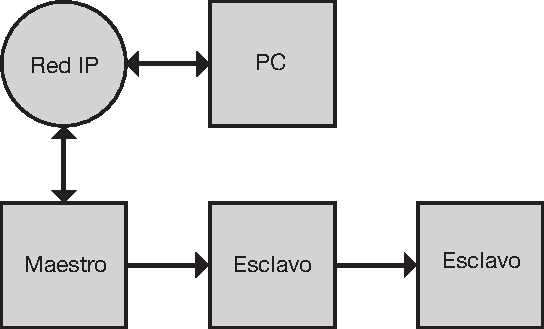
\includegraphics[scale=1]{imagenes/esquema-general.pdf}
	\caption{Esquema general entre todos los componentes del sistema.}
	\label{fig:diagrama-bloques-general}
\end{figure}

En la figura \ref{fig:diagrama-bloques-general}, se observa en primer lugar la PC, a partir de ahora \enquote{cliente}. Esta es la componente que interactúa directamente con el usuario.

Conectando su computadora a la misma red que se encuentra vinculado el cartel, el cliente puede, por medio de dicha aplicación, enviar los comandos para que el sistema satisfaga sus necesidades.

Por medio del protocolo de comunicación WiFi y la pila de protocolos TCP/IP, los datos llegan hacia el microcontrolador que se encuentra en el módulo maestro. Cabe destacar que el protocolo de red que encapsula las distintas acciones que el usuario puede realizar se trata de un protocolo binario personalizado que ha sido diseñado específicamente para este proyecto y se explica en mayor detalle en el apéndice \ref{sec:protocolo}.
Dicho protocolo se implementa tanto del lado de la aplicación de PC, como del microcontrolador que controla el cartel. La información se transmite cifrada.

Tras recibir y decifrar los datos, el microcontrolador procesa la información y la transmite vía protocolo serie sincrónico hacia el primer driver MAX7219 que controla la primera matriz de LEDs.

Resulta necesario aclarar que cada módulo esclavo posee un MAX7219 y la información que le proporciona el microcontrolador se transmite sólo al primero de ellos. Luego esta información se desplaza entre los diferentes MAX7219 utilizando determinados pines de dicho módulo.
De esta forma, el microcontrolador solo mantiene una conexión física directa con el primer esclavo, con lo cual la señal digital se regenera en cada eslabón.

Finalmente, cada módulo esclavo proyecta en su respectiva matriz de LEDs la información suministrada por el maestro, de manera que se muestra el mensaje que el cliente ha enviado inicialmente por medio de la aplicación de PC.

Cabe destacar que la comunicación entre la aplicación de PC y el cartel es bidireccional, debido a que todas las operaciones que el cliente realice, necesitan de una respuesta.
En algunos casos, dicha respuesta es solo para indicar éxito o error, mientras que en otros casos el usuario recibe parámetros de configuración y las credenciales de red a las que el sistema se encuentra actualmente conectado.

\subsection{Módulo maestro}
Como se mencionó anteriormente, este módulo se encarga de procesar los datos enviados desde el cliente a fin de convertir dicha información en comandos que posteriormente son transmitidos hacia los diferentes esclavos que componen el cartel.

Para realizar esta operación, el módulo maestro requiere de un microcontrolador que sea capaz de conectarse a una red WiFi, a fin de poder obtener las peticiones que el usuario realice por medio de la aplicación de PC.

El microcontrolador, entonces, debe recibir los pedidos a través de la red y convertirlos en paquetes que puedan ser interpretados por los drivers de LEDs que se ubican en cada uno de los esclavos.

Para el presente proyecto, se opta por el microcontrolador ESP8266EX de Espressif que posee funcionalidades para operar con redes WiFi y conexiones seguras. Además tiene un procesador con una frecuencia aproximada de 80 Mhz de prestaciones suficientes para los requerimientos de este sistema. En el apartado \ref{sec:microcontrolador} se detallan las especificaciones y diagramas en bloque de este dispositivo electrónico.

Para la elección de los drivers encargados de manejar las matrices de LEDs, se opta por el MAX7219 por ser un dispositivo mundialmente conocido en la industria del hardware, cuyas principales aplicaciones donde se utiliza es para el control de dispositivos LEDs de 7 segmentos de hasta 8 dígitos, pantallas de gráficos de barras o incluso 64 LEDs individuales, dispuestos de forma matricial.
Las especificaciones de este circuito integrado se encuentran detalladas en el apartado \ref{sec:max7219}.

El principal inconveniente que se produce al momento en que interactúan el NodeMCU (ESP8266EX) con los MAX7219 es que manejan diferentes niveles de tensiones lógicas. El primero trabaja a 3.3 V, mientras que los segundos a 5 V. Para ello, es necesario agregar en el módulo maestro un circuito de conversión de señal realizado a partir de transistores. Esto se explica más en detalle en la sección \ref{sec:transistores}.

Tanto el microcontrolador como los drivers de LEDs elegidos para este sistema utilizan una alimentación de 5 V continua. Por este motivo es necesario una interfaz de entrada hacia el módulo maestro de donde puedan obtener la tensión necesaria los distintos dispositivos electrónicos que conforman la totalidad del cartel. Esto se explica en detalle en la sección \ref{sec:alimentacion}.

El microcontrolador almacena los parámetros de configuración previamente establecidos desde la aplicación de PC. Uno de ellos es la red WiFi a la que debe conectarse. Para evitar que el cartel sea inaccesible por una mala configuración accidental de la red, se añadió al diseño un pulsador de RESET, el cual, al ser presionado durante 5 segundos, reestablece los parámetros de configuración por defecto y reinicia el módulo maestro, por lo tanto también el cartel.

Por otro lado, resulta necesario comunicar al firmware del microcontrolador la cantidad de carteles que conforman el eslabón de esclavos. Para esto se utiliza un conjunto de jumpers que codifican la cantidad de carteles conectados, de manera que el usuario pueda agregar o quitar carteles sin necesidad de volver a cargar el firmware modificado. Ésto se explica en mayor detalle en el manual de usuario (ver sección \ref{sec:manual-usuario}).

En los siguientes apartados se describiran las partes que conforman el diseño del circuito del módulo maestro, dividido de la manera que muestra la figura \ref{fig:esquematico-master-anotado}.

\begin{figure}[ht!]
	\centering
	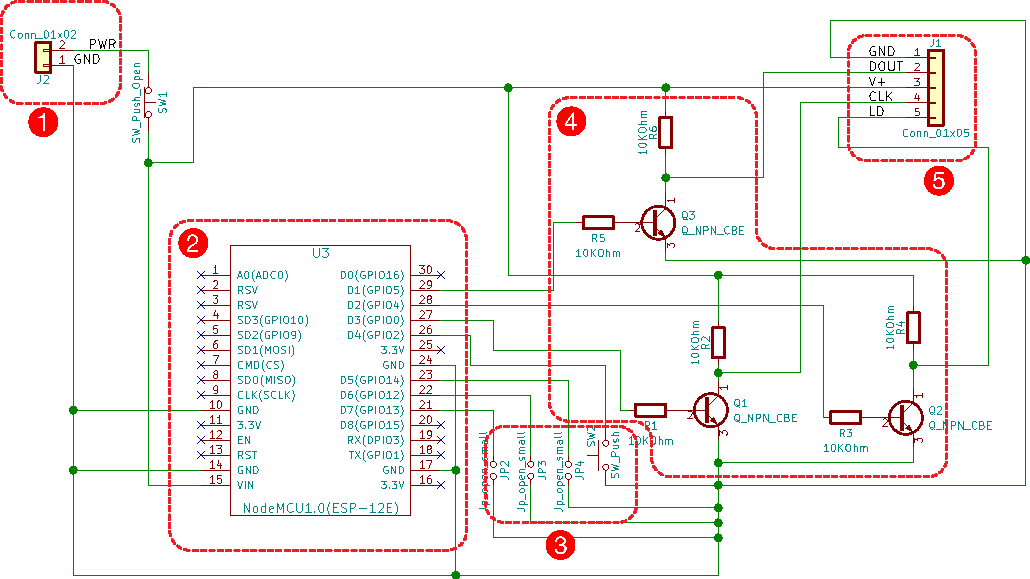
\includegraphics[width=\linewidth]{imagenes/esquematico-master-anotado.pdf}
	\caption{Esquemático del módulo maestro, dividido en subcircuitos.}
	\label{fig:esquematico-master-anotado}
	% Ojo con el orden, tiene que coincidir con el orden en la imagen.
	\begin{enumerate}
		\item Ficha de alimentación (ver sección \ref{sec:alimentacion}).
		\item Microcontrolador ESP8266EX (ver sección \ref{sec:microcontrolador}).
		\item Componentes de interacción directa con usuario (ver sección \ref{sec:jumpers-rst}).
		\item Circuito de conversión de niveles lógicos (ver sección \ref{sec:transistores}).
		\item Ficha de conexión a esclavo (ver sección \ref{sec:ficha-esclavo}).
	\end{enumerate}
\end{figure}

\subsubsection{Alimentación} \label{sec:alimentacion}
El cartel requiere una alimentación de 5V de corriente continua. Para esto se expone un conector hembra (de 5.5mm x 2.1mm), el cual se conecta a un transformador externo de 220V AC a 5V DC. El sistema no posee batería de ningún tipo.

Esta tensión permite alimentar tanto al microcontrolador ESP8266EX como a todos los drivers MAX7219 que posee el circuito, incluidas las matrices de LEDs que tiene cada uno asociada.

En la sección \ref{part:ensayos} se agrega más información respecto del consumo que posee el  circuito completo y los diferentes mecanismos que se realizaron para obtener dichos parámetros.

\subsubsection{Microcontrolador} \label{sec:microcontrolador}
El componente central en el módulo maestro es el microcontrolador ESP8266EX, el cual se encuentra contenido en un módulo AI-Thinker ESP-12E (figura \ref{fig:foto-esp12e}), el cual está montado sobre un módulo NodeMCU que le provee de regulación de tensión y un conversor de serie TTL a USB. El ESP8266EX es un SoC (\emph{System on Chip}) de la empresa Espressif. El módulo NodeMCU es hardware libre, sin embargo, el ESP12E y el ESP8266EX no lo son.\cite{NodeMCU}

Es importante tener en cuenta que el sistema no integra en su hardware directamente ni el ESP12E ni el ESP8266EX, sino que utiliza el NodeMCU, cuya asignación de pines se puede ver en la figura \ref{fig:nodemcu-pinout}.

\begin{figure}[ht!]
	\begin{center}
		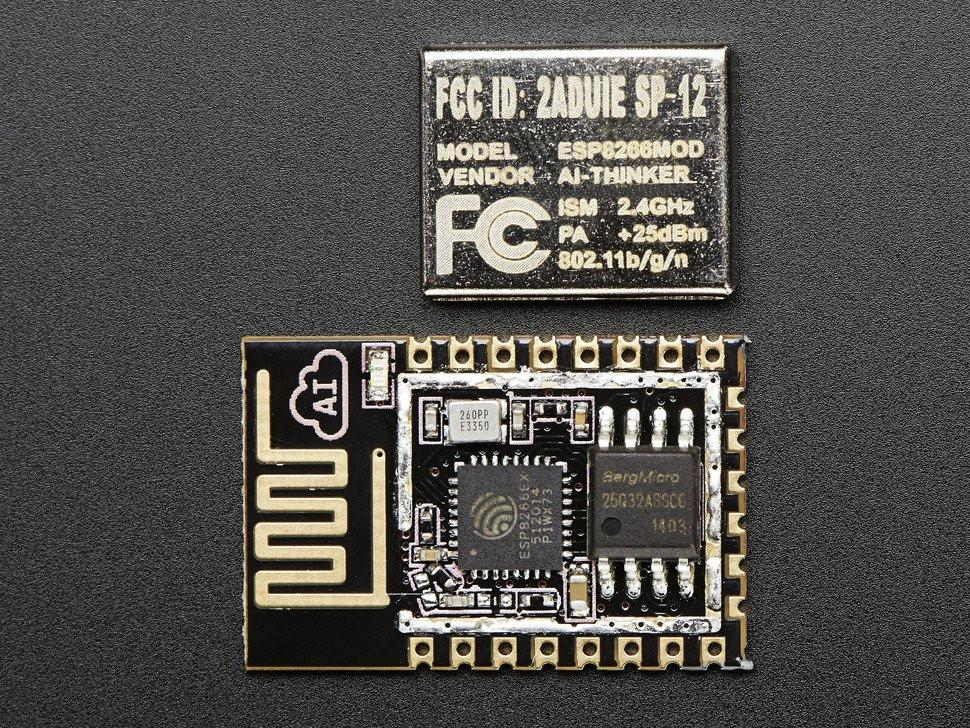
\includegraphics[width=0.4\textwidth]{imagenes/esp12e-foto.jpg}
		\caption{Foto del módulo ESP12E sin su cubrimiento.}
		\label{fig:foto-esp12e}
	\end{center}
\end{figure}

\begin{figure}[ht!]
	\begin{center}
		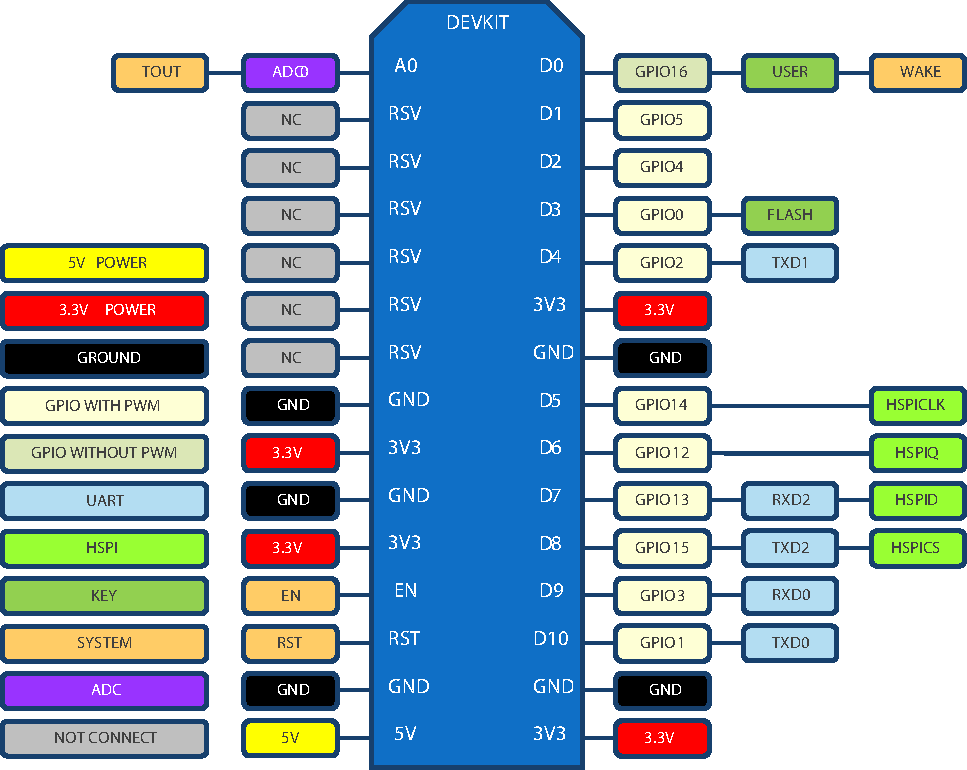
\includegraphics[width=0.85\textwidth]{imagenes/nodemcu-pinout.pdf}
		\caption{Asignación de pines del NodeMCU.}
		\label{fig:nodemcu-pinout}
	\end{center}
\end{figure}

Utilizando la figura \ref{fig:esquematico-master-anotado} y la asociación de pines de la figura \ref{fig:nodemcu-pinout}, es posible aclarar que los pines GPIO12, GPIO13 y GPIO14 se utilizan para la conexión de los jumpers. Mientras que el pin GPIO2 para el botón de RESET. Por otra parte los pines GPIO0, GPIO4 y GPIO5 se utilizan para las señales CLK, LOAD y DATAIN necesarias para la comunicación entre el microcontrolador y los drivers MAX7219.

El chip ESP8266EX combina un microcontrolador Tensillica Xtensa L106, un RISC de 32 bits corriendo a 80 Mhz, con funcionalidad WiFi. \cite{ESP8266Datasheet} El chip tiene memoria ROM con firmware no removible, y puede correr programas almacenados en flash externa. Para poder usar todas sus funcionalidades, se debe programar sobre firmware privativo desarrollado por Espressif, esto implica que el programa de usuario corre en simultáneo con el firmware (utilizando funciones disponibilizadas por el firmware) y el uso de la memoria de trabajo está sujeto a la versión del firmware. Según el datasheet del ESP8266EX, el usuario puede esperar tener disponible 50 KiB de RAM para alocar variables globales o utilizando la heap.

El firmware de Espressif para el ESP8266EX implementa por completo la pila de protocolos TCP/IP, el protocolo 802.11 b/g/n/e/i y Wi-Fi Direct.

El ESP8266EX está diseñado con tecnologías de manejo de consumo y está dirigida a dispositivos móviles, dispositivos \emph{wearables} y para aplicaciones de internet de las cosas (IoT).

El hardware del microcontrolador opera en tres modos: modo activo, \emph{sleep} y \emph{deep-sleep}. Sin embargo, para este proyecto en particular, donde el dispositivo no tiene batería y está conectado permanentemente a la red eléctrica, no se utiliza ningún modo aparte del activo.

El microcontrolador provee 17 pines GPIO. El firmware permite emular mediante \emph{bit-banging} los protocolos SPI, SDIO, I2C, I2S y UART en cualquier pin que el programador elija y esté disponible para su uso. No todos los pines pueden ser utilizados libremente, ya que algunos de ellos están conectados a la memoria flash. El firmware también incluye una implementación software de PWM, ya que el microcontrolador no posee hardware de PWM real.

Se puede ver un diagrama de bloques del ESP8266EX en la figura \ref{fig:diagrama-bloques-esp8266ex}.

\begin{figure}[htp!]
	\centering
	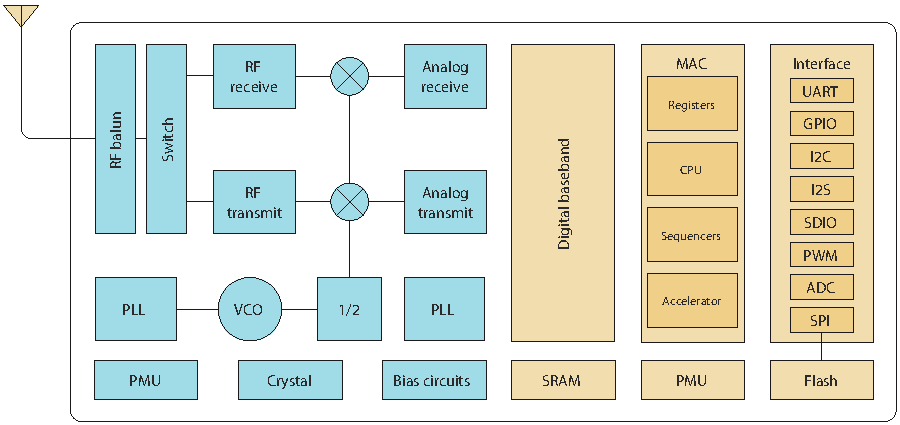
\includegraphics[width=\linewidth]{imagenes/diagrama-bloques-esp8266.pdf}
	\caption{Diagrama de bloques del Espressif ESP8266EX.}
	\label{fig:diagrama-bloques-esp8266ex}
\end{figure}

Como se mencionó anteriormente, se necesita de flash externa para correr programas. El módulo ESP-12S se encarga de proveer al ESP8266EX 4 MiB de memoria flash.

\subsubsection{Jumpers y botón de Reset} \label{sec:jumpers-rst}
Esta sección del circuito aglomera las componentes con las cuales el usuario (especificamente, el usuario encargado de mantener la operacion del cartel) va a interactuar directamente.

El pulsador de Reset es un pulsador normalmente abierto, que conecta el pin GPIO2 del microcontrolador a la masa. El pin GPIO2 está configurado como entrada, con lo cual es necesario un circuito de pull-up para que su nodo circuital no tenga un valor lógico indefinido. Para esto se utiliza el pull-up interno del microcontrolador, equivalente al de la figura \ref{fig:pull-up}.

Los jumpers, de manera similar, conectan los pines GPIO13, GPIO12, GPIO14 a masa. También utilizan el pull-up interno del microcontrolador.

\begin{figure}[htp!]
	\centering
	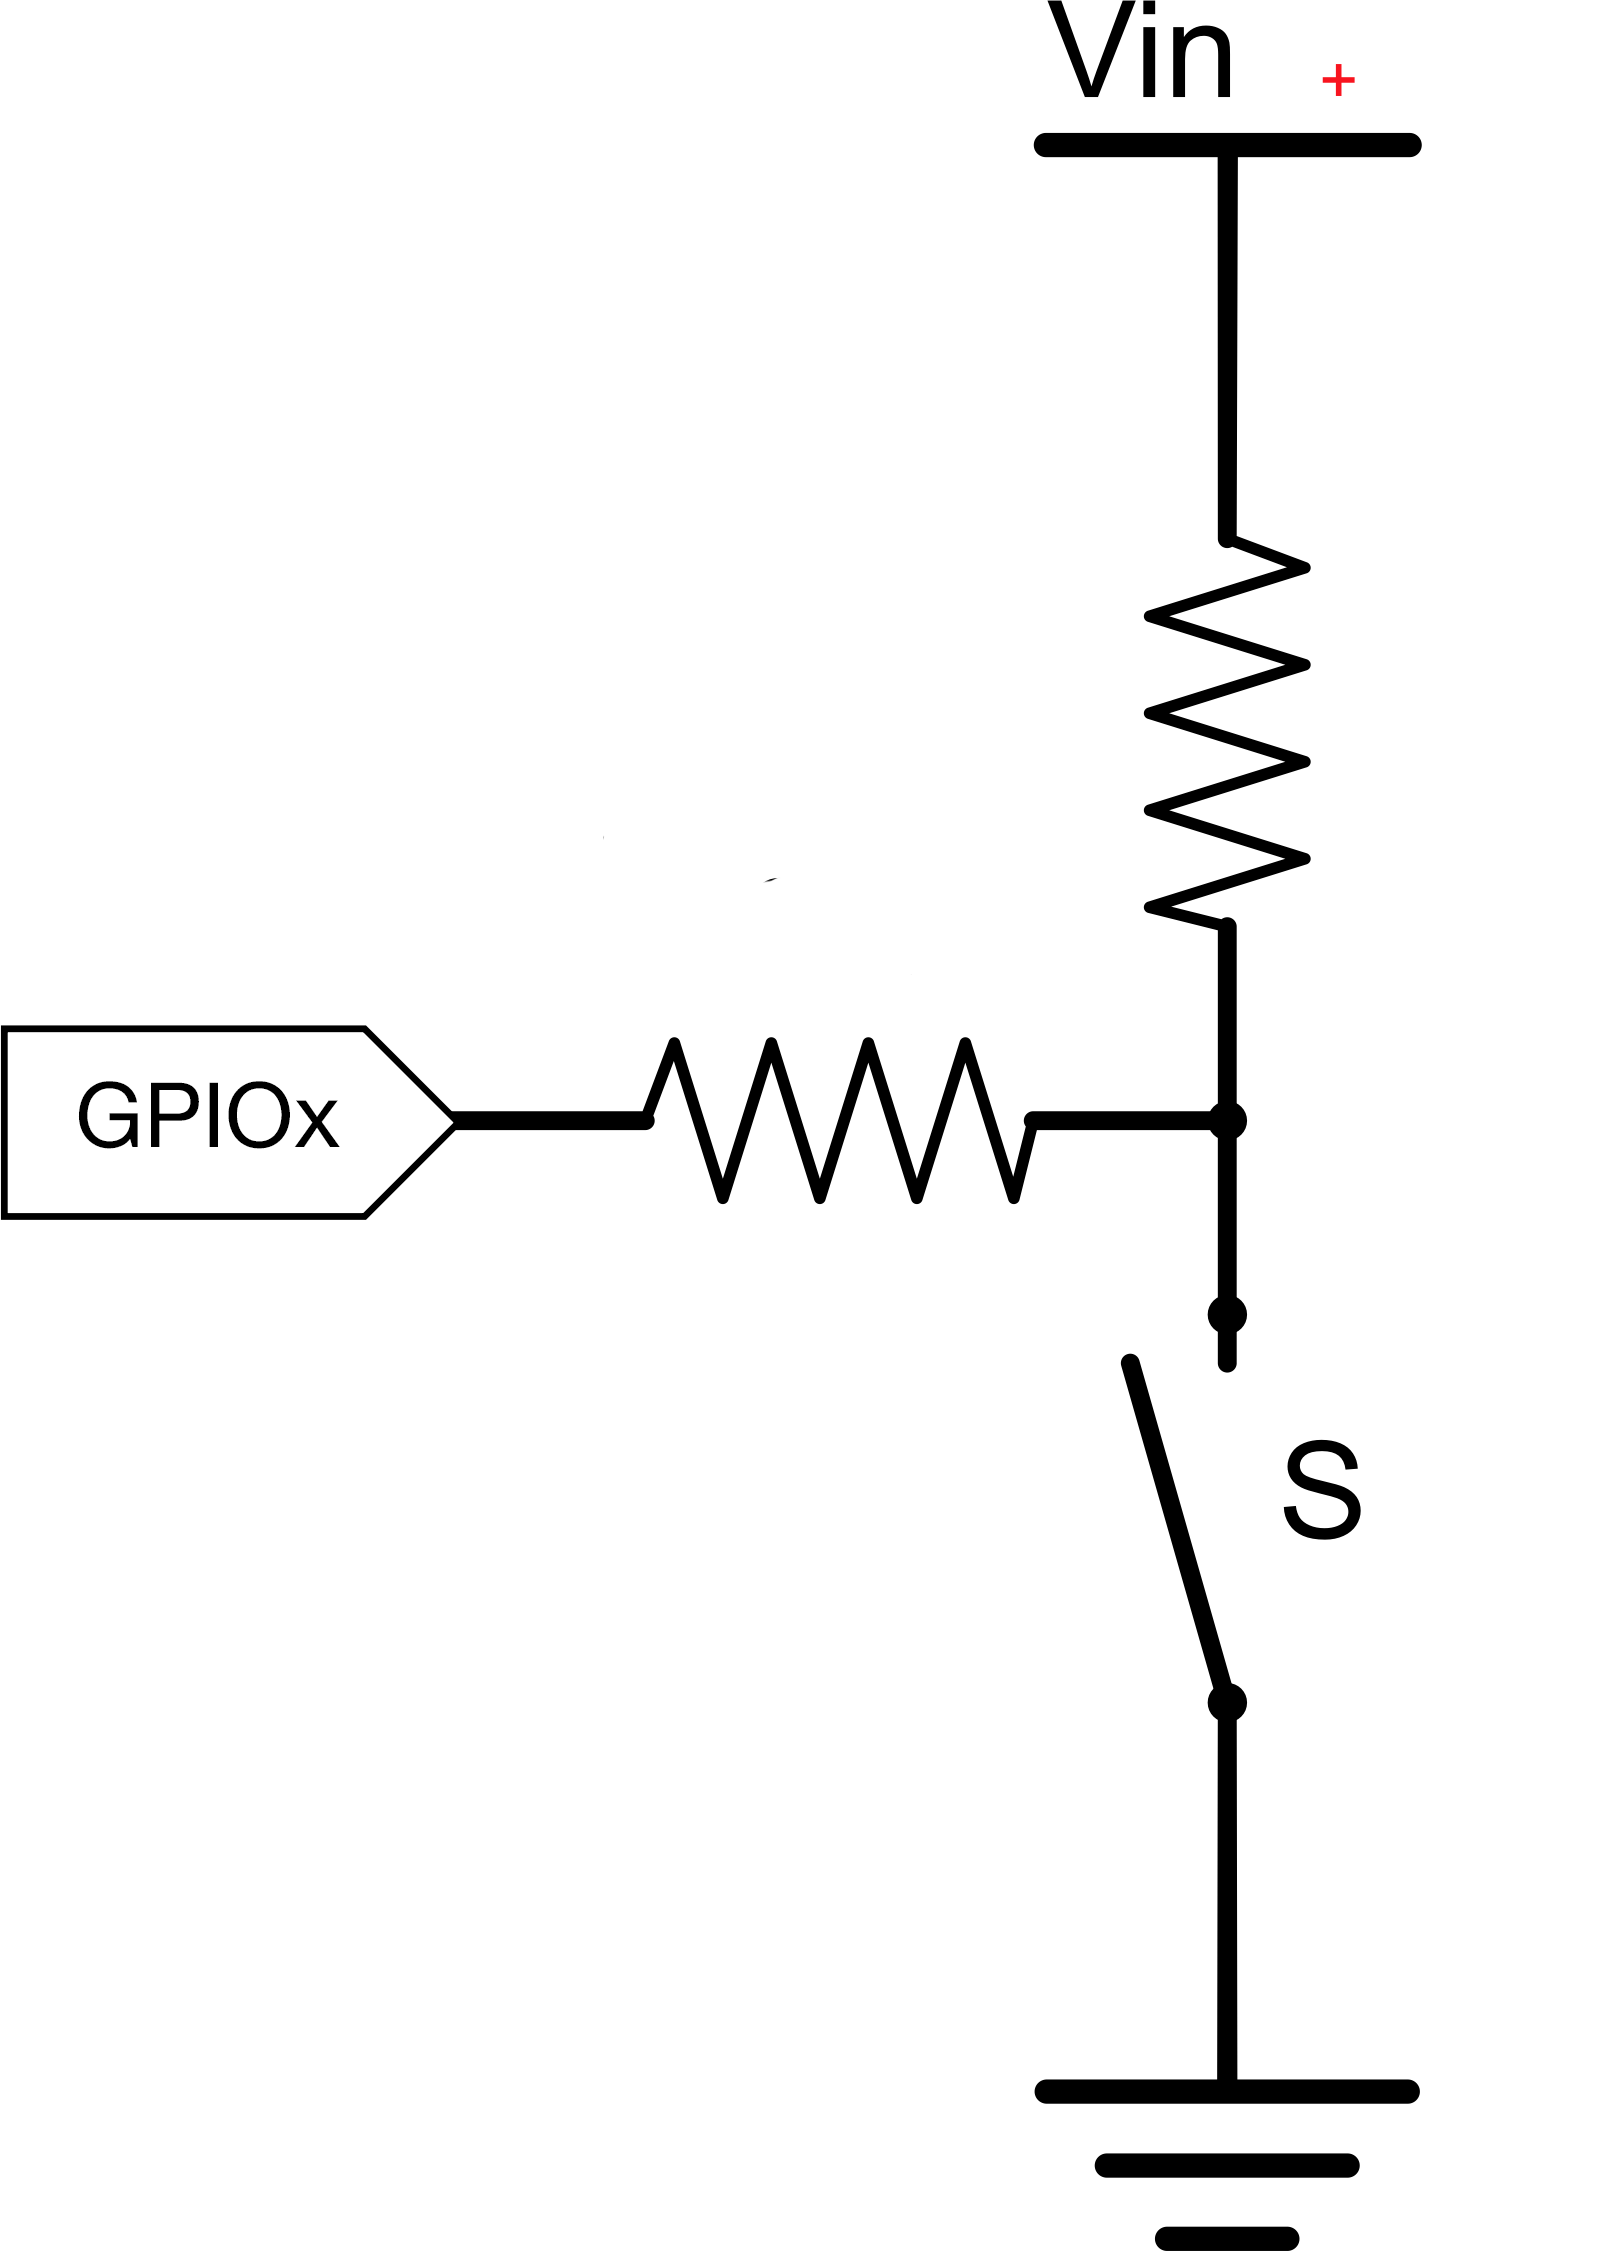
\includegraphics[height=5cm]{imagenes/pullup_resistor.png}
	\caption{Circuito de pull-up genérico, donde el elemento S representa tanto un pulsador como un jumper.}
	\label{fig:pull-up}
\end{figure}

\subsubsection{Circuito de conversión de niveles} \label{sec:transistores}
Como el microcontrolador transmite los datos con un valor alto de 3.3V, es necesario convertir estas señales para que este dentro de los rangos con los que trabaja el MAX7219. La solución por la cual se optó fue incorporar transistores configurados de manera que ante una entrada de 0V, produzcan 5V y ante una entrada de 3.3V, produzcan 0V (aproximado). 

Se conectan tres transistores NPN al circuito del módulo maestro, uno para cada señal: DATAIN, LOAD, CLK, que corresponde a los pines GPIO5, GPIO4 y GPIO0 del microcontrolador respectivamente. 
Se puede observar en la figura \ref{fig:transistors} la conexión de cada transistor con sus respectivas resistencias. 

Esta solución tiene como consecuencia el hecho de que la señal digital se invierte, para eliminar este problema, fue necesario modificar el firmware del cartel para invertir el valor lógico de sus salidas.

Los transistores utilizados en el prototipo final son los 2N2369. %(http://www.pci-card.com/2n2369.pdf)
El pin 2 corresponde a la base, donde se conecta las señales previamente enumeradas. Por otro lado el colector es el pin 1 donde se conecta VCC mientras que el emisor el pin 3 al que se le conecta GND (ver figura \ref{fig:transistors}).

Finalmente la salida se conecta desde el emisor, y se encuentra invertida respecto a la entrada que se origina por la base.

\begin{figure}[ht!]
	\centering
	\begin{center}
		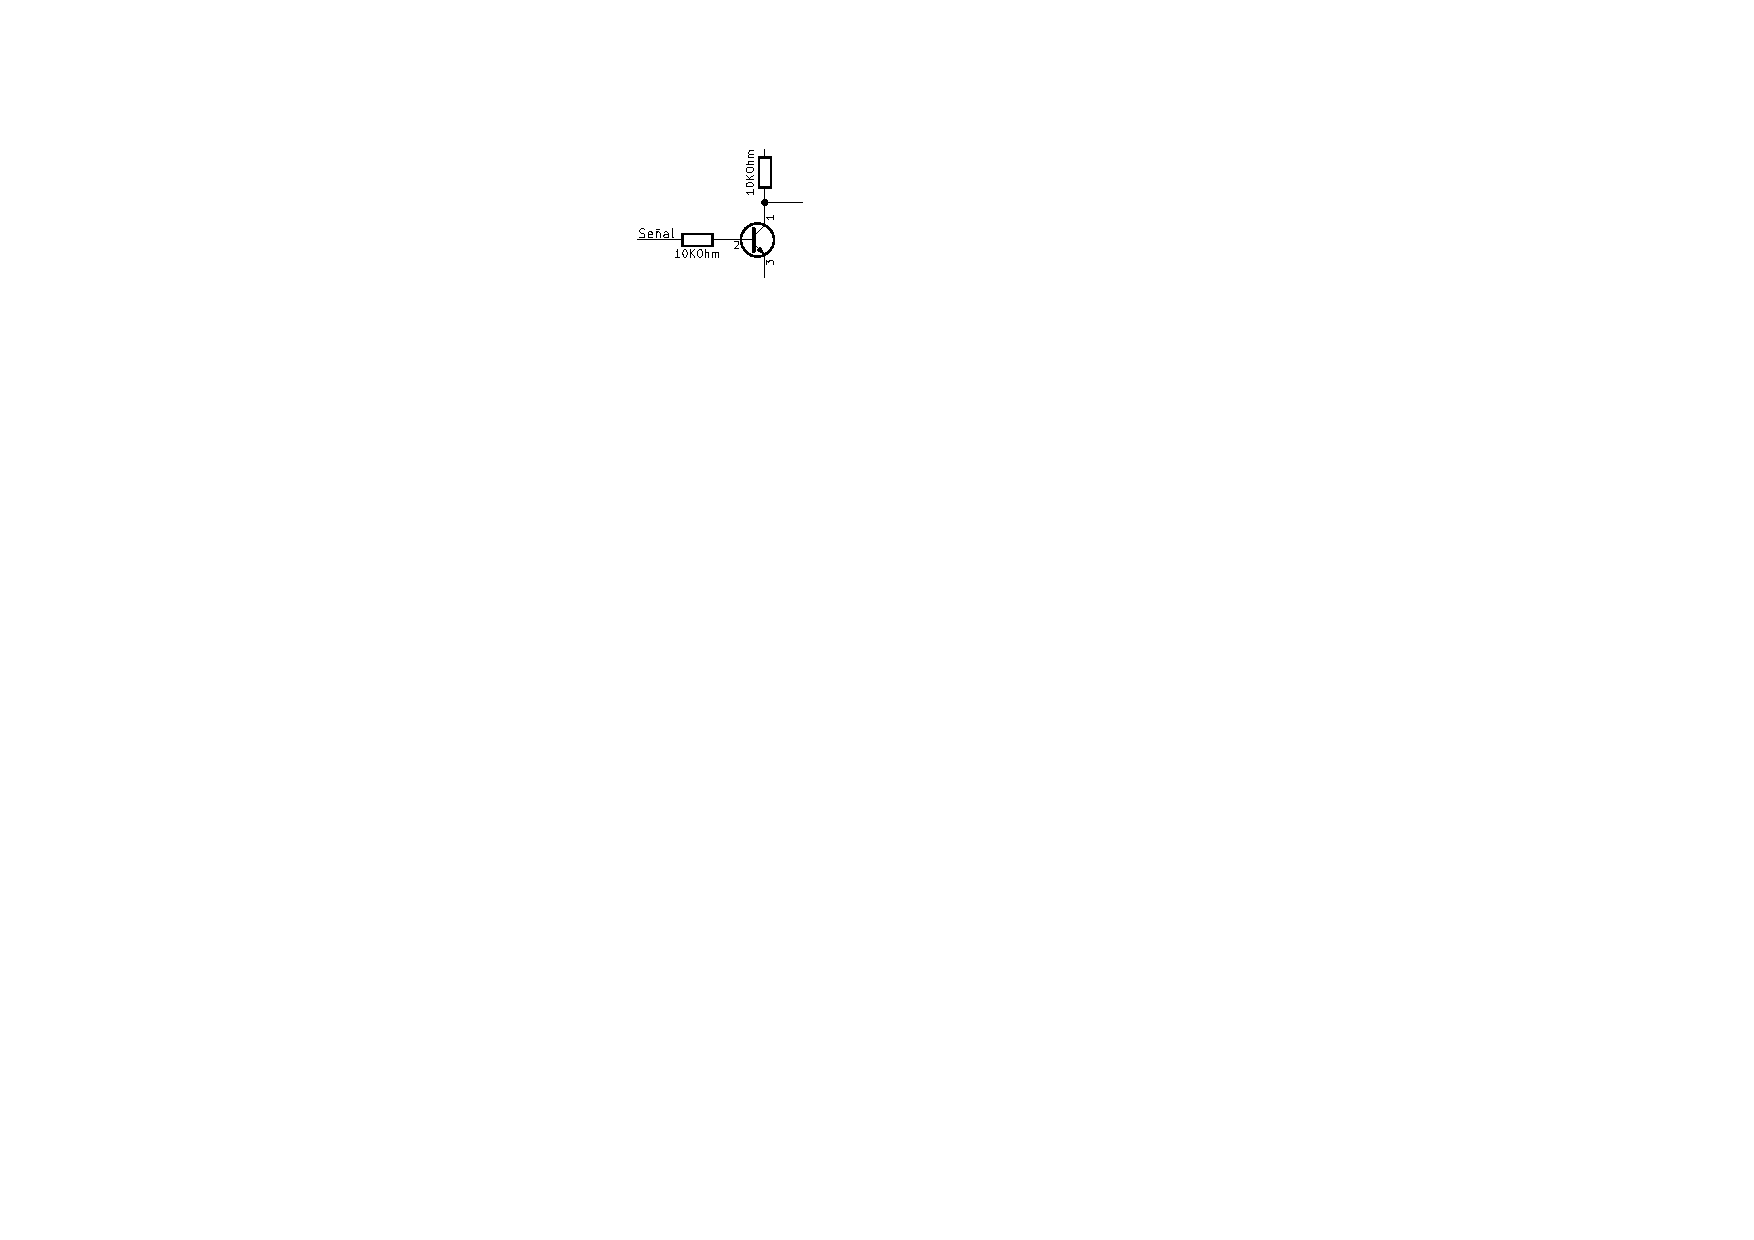
\includegraphics[scale=2]{imagenes/hw/transistor.pdf}
		\caption{Conexión de un transistor junto con los valores de las resistencias.}
		\label{fig:transistors}
	\end{center}
\end{figure}

\pagebreak
\subsubsection{Comunicación con el primer esclavo} \label{sec:ficha-esclavo}
En esta porción del circuito se tiene la interfaz de conexión al primer esclavo. 
Que luego en el diseño del PCB terminará siendo una ficha.

El maestro expone todas las señales que necesita el primer esclavo para recibir los comandos que envía el microcontrolador.
Dichas señales corresponden, en primer lugar, a los 5V y GND provenientes de la fuente.

Adicionalmente, el primer esclavo recibe las señales de CLK, LATCH y DATAIN, ya convertidas a valores lógicos de 5V. Para más información revisar la sección \ref{sec:transistores}.

\subsubsection{Esquemático final}
Habiendo descrito por partes el esquemático del módulo maestro, se muestra en la figura \ref{fig:esquematico-master} el circuito completo sin anotaciones.

\begin{figure}[ht!]
	\centering
	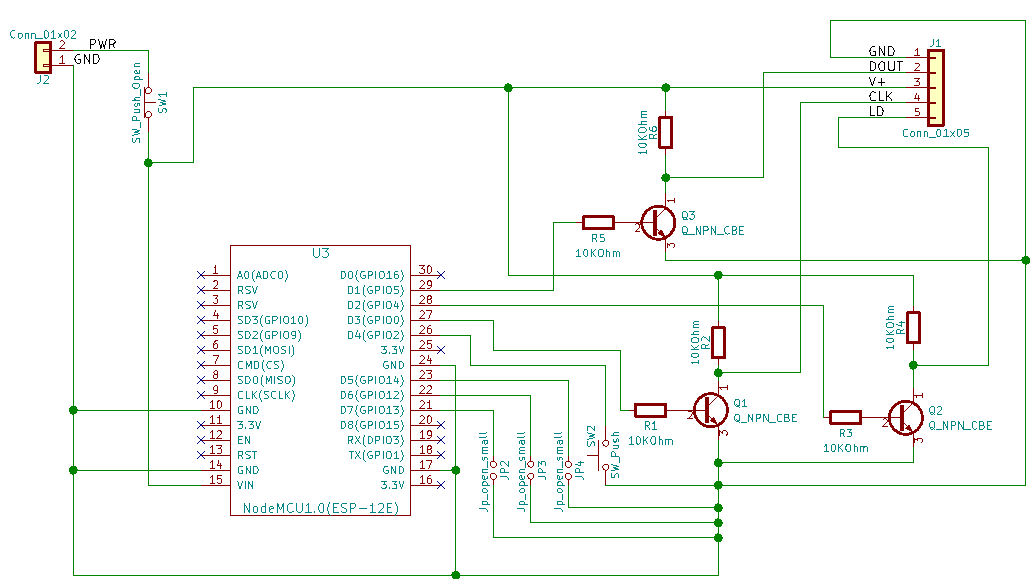
\includegraphics[width=\linewidth]{imagenes/esquematico-master.pdf}
	\caption{Esquemático del módulo maestro.}
	\label{fig:esquematico-master}
\end{figure}

\subsubsection{Diseño de PCB}

El módulo maestro emite el mensaje hacia los módulos esclavo, sin encargarse especificamente de su visualización.

El ESP8266EX es el componente más importante de este módulo, ya que se encarga tanto de comunicarse con la computadora del usuario para la configuración del mensaje como de emitir el mensaje a los módulos esclavo.

El PCB contará con las pistas necesarias para cerrar el circuito electrónico que unirá los componentes de este módulo.

Los tres transistores NPN actuarán en corte y saturación con el fin de convertir las señales de datos del NodeMCU, pasando las mismas de 3.3 V (salida del NodeMCU, valor que pese a funcionar en la práctica estaba fuera de los márgenes aceptados en las entradas del MAX7219 según su hoja de datos) a 5V (valor válido y seguro de funcionamiento). Las resistencias adaptarán los valores de tensión y corriente del circuito de forma pasiva.

Los jumpers permitirán indicar en la configuración del sistema la cantidad de módulos esclavo a utilizar, representando en función del sistema numérico basado en base 2 presentado anteriormente.

El jack con bornera permitirá alimentar al circuito mediante un cable de alimentación con una ficha genérica o bien a través de un método alternativo que se conecte en la bornera provista.

La tecla rocker switch controlará que se provea la alimentación al circuito, permitiendo encender o apagar el cartel manualmente. Dos tiras de 15 pines hembra serán empleadas para poder conectar el NodeMCU al PCB sin necesidad de soldarlo, facilitando su reutilización en caso de ser necesaria. Finalmente una tira de 5 pines macho permitirá conectar el módulo a un módulo esclavo para la transmisión de las señales de datos y alimentación.

Se puede ver en la figura \ref{fig:pcb-master} el diseño final de la PCB del maestro.
\begin{figure}[ht!]
	\centering
	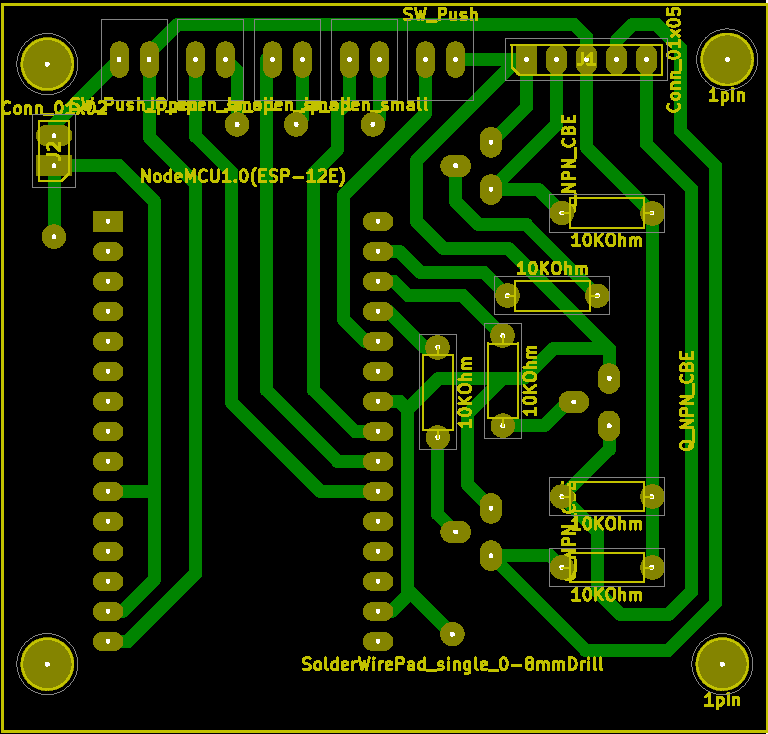
\includegraphics[width=0.7\linewidth]{imagenes/pcb-master.pdf}
	\caption{PCB del módulo maestro.}
	\label{fig:pcb-master}
\end{figure}

\clearpage
\subsection{Módulo esclavo}
Un módulo esclavo posee un driver de LEDs conocido como MAX7219, que es el componente principal de este subsistema y se encarga de controlar la matriz de 8x8 LEDs que tiene asociada.

Este módulo recibe los comandos que el microcontrolador del maestro le envía por medio de un protocolo de comunicación serie sincrónico. La interfaz de conexión comprende 3 señales. Estas son CLK, LATCH y DATAIN, además de la conexión de la alimentación y masa.

Cabe destacar que, físicamente, un esclavo posee dos interfaces de conexión como las que se describió en el párrafo anterior. Una se utiliza como puerto de entrada, mientras que la otra como de salida.

La necesidad de colocar dos interfaces surge del hecho que el maestro se conecta con un primer esclavo, y éste se conecta en cadena con otros esclavos como observa en la figura \ref{fig:dibujo-real}.

Un esclavo puede conectarse a través de su puerto de entrada con el módulo maestro, en caso de ser el primero de la cadena. En su defecto, un esclavo puede conectarse con un esclavo anterior, del cual recibe las señales propagadas desde el maestro.

A su vez, se interconecta, a través de su interfaz de salida con el módulo esclavo siguiente, permitiendo que la información proveniente del maestro fluya a lo largo de todo el sistema.

Adicionalmente, el esclavo posee una interfaz de comunicación que permite conectar el MAX7219 con su respectiva matriz de LEDs. Para esto se exponen 8 pines correspondientes a las filas de la matriz y 8 para las columnas.

\subsubsection{Esquemático general}
El esquemático general del módulo esclavo se presenta en la figura \ref{fig:esquematico-esclavo}.
Además se enumeran y describen los diferentes subcircuitos que lo componen en relación a lo descripto en la sección anterior.
Dichos subcircuitos cumplen una función específica y aparecen enumerados al pie de la imagen.

\begin{figure}[ht!]
	\centering
	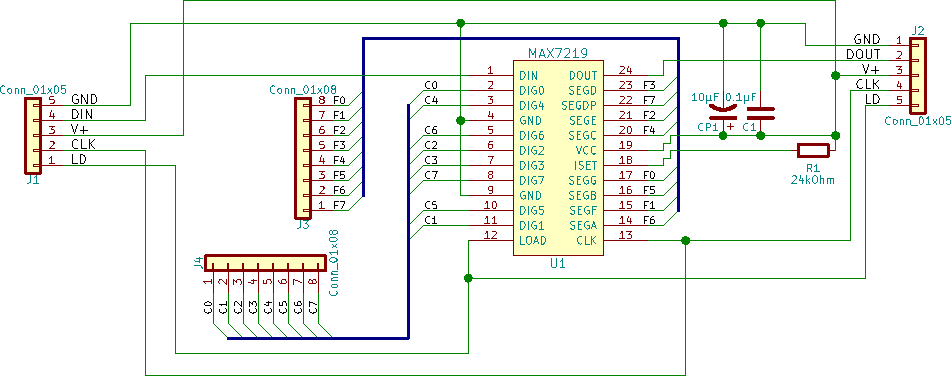
\includegraphics[width=\linewidth]{imagenes/esquematico-slave.pdf}
	\caption{Esquemático del módulo esclavo, dividido en subcircuitos.}
	\label{fig:esquematico-esclavo}
\end{figure}

\begin{enumerate}
	\item Driver de LEDs MAX7219: Este dispositivo electrónico es el componente principal del módulo esclavo por lo que en la sección \ref{sec:max7219} se abordan, más en detalle, las características principales del mismo.
	\item Interfaz de entrada: se comparten las líneas VCC, GND, CLK, DATAIN y LATCH del anterior módulo en la cadena, pudiendo corresponderse tanto al maestro como a otro esclavo.
	\item Interfaz de salida: se comparten las líneas de VCC, GND, CLK, DATAOUT y LATCH del próximo módulo esclavo en la cadena.
	\item Interfaz de conexión con las filas de la matriz: En la sección \ref{sec:matriz-leds} se hace un especial énfasis en la comunicación entre la matriz de 8x8 LEDs con el MAX7219.
	\item Interfaz de conexión con las columnas de la matriz: Ver sección \ref{sec:matriz-leds}.
\end{enumerate}

\subsubsection{MAX7219}\label{sec:max7219}
El MAX7219 es un controlador compacto, de entrada y salida en serie de cátodo común que conectan, indirectamente, microcontroladores a LEDs numéricos de siete segmentos de hasta ocho dígitos, pantallas de gráfico de barras o, en este caso, 64 LED individuales dispuestos de forma matricial. Se incluye en el chip, un decodificador BCD, circuitos de multiplexación, controladores de segmentos y dígitos, y una RAM estática de 8x8 que almacena cada número, o en este caso, mapas de bits. Solo se necesita una resistencia externa para configurar la corriente para todos los LEDs.

Las matrices individuales se pueden actualizar sin reescribir toda la pantalla.

Su alimentación V\texttt{+} debe estar entre 4 y 5.5 Volts para su correcto funcionamiento. En cambio los voltaje de las entradas lógicas tienen una restricción de que un valor alto como mínimo debe ser 3.5V y un valor bajo debe ser como máximo 0.8V.

Las características principales que posee el chip integrado se enumeran a continuación:
\begin{itemize}
	\item Interfaz serie de 10 MHz.
	\item Control de segmento LED individual.
	\item Selección de dígitos Decode / No-Decode.
	\item Apagado de baja potencia de 150 microA (datos retenidos).
	\item Control de brillo digital y analógico.
	\item Pantalla borrada al encenderse (todos los LEDs apagados).
	\item Unidad de visualización LED de cátodo común.
	\item SPI, QSPI, interfaz serie Microwire paquetes DIP y SO de 24 pines.
\end{itemize}

La disposición de los pines del MAX7219 se puede observar en la figura \ref{fig:MAX-pines} y la descripción de cada uno en la tabla \ref{table:MAX-pines}.

Es necesario prestar atención en el conexionado con respecto a los pines de tierra (GND) ya que ambos deben estar conectados para el driver pueda funcionar correctamente, ambas están al lado izquierdo de la figura \ref{fig:MAX-pines} (Pin 4 y 9).

Por otro lado, el MAX7219 tiene un pin denominado DOUT (pin 24) se utiliza para encadenar varios MAX7219 y de esta forma pasar la información al que esta directamente conectado, éste pin nunca tiene alta impedancia.

Los otros pines más reelevantes de este driver son los que utiliza el microcontrolador para transmitir los comandos requeridos. Estos son el pin DIN (pin 1)
donde ingresan los datos al MAX7219. Adicionalmente se encuentra el LOAD (pin 12) requerido para indicarle a este dispositivo, que los últimos 16 bits recibidos deben ser cargados. Finalmente se encuentra la señal de CLCK (pin 13) que se utiliza para la transmisión sincrónica entre el maestro (microcontrolador) y los esclavos (drivers de LEDs).

\begin{figure}[htp!]
	\centering
	\begin{center}
	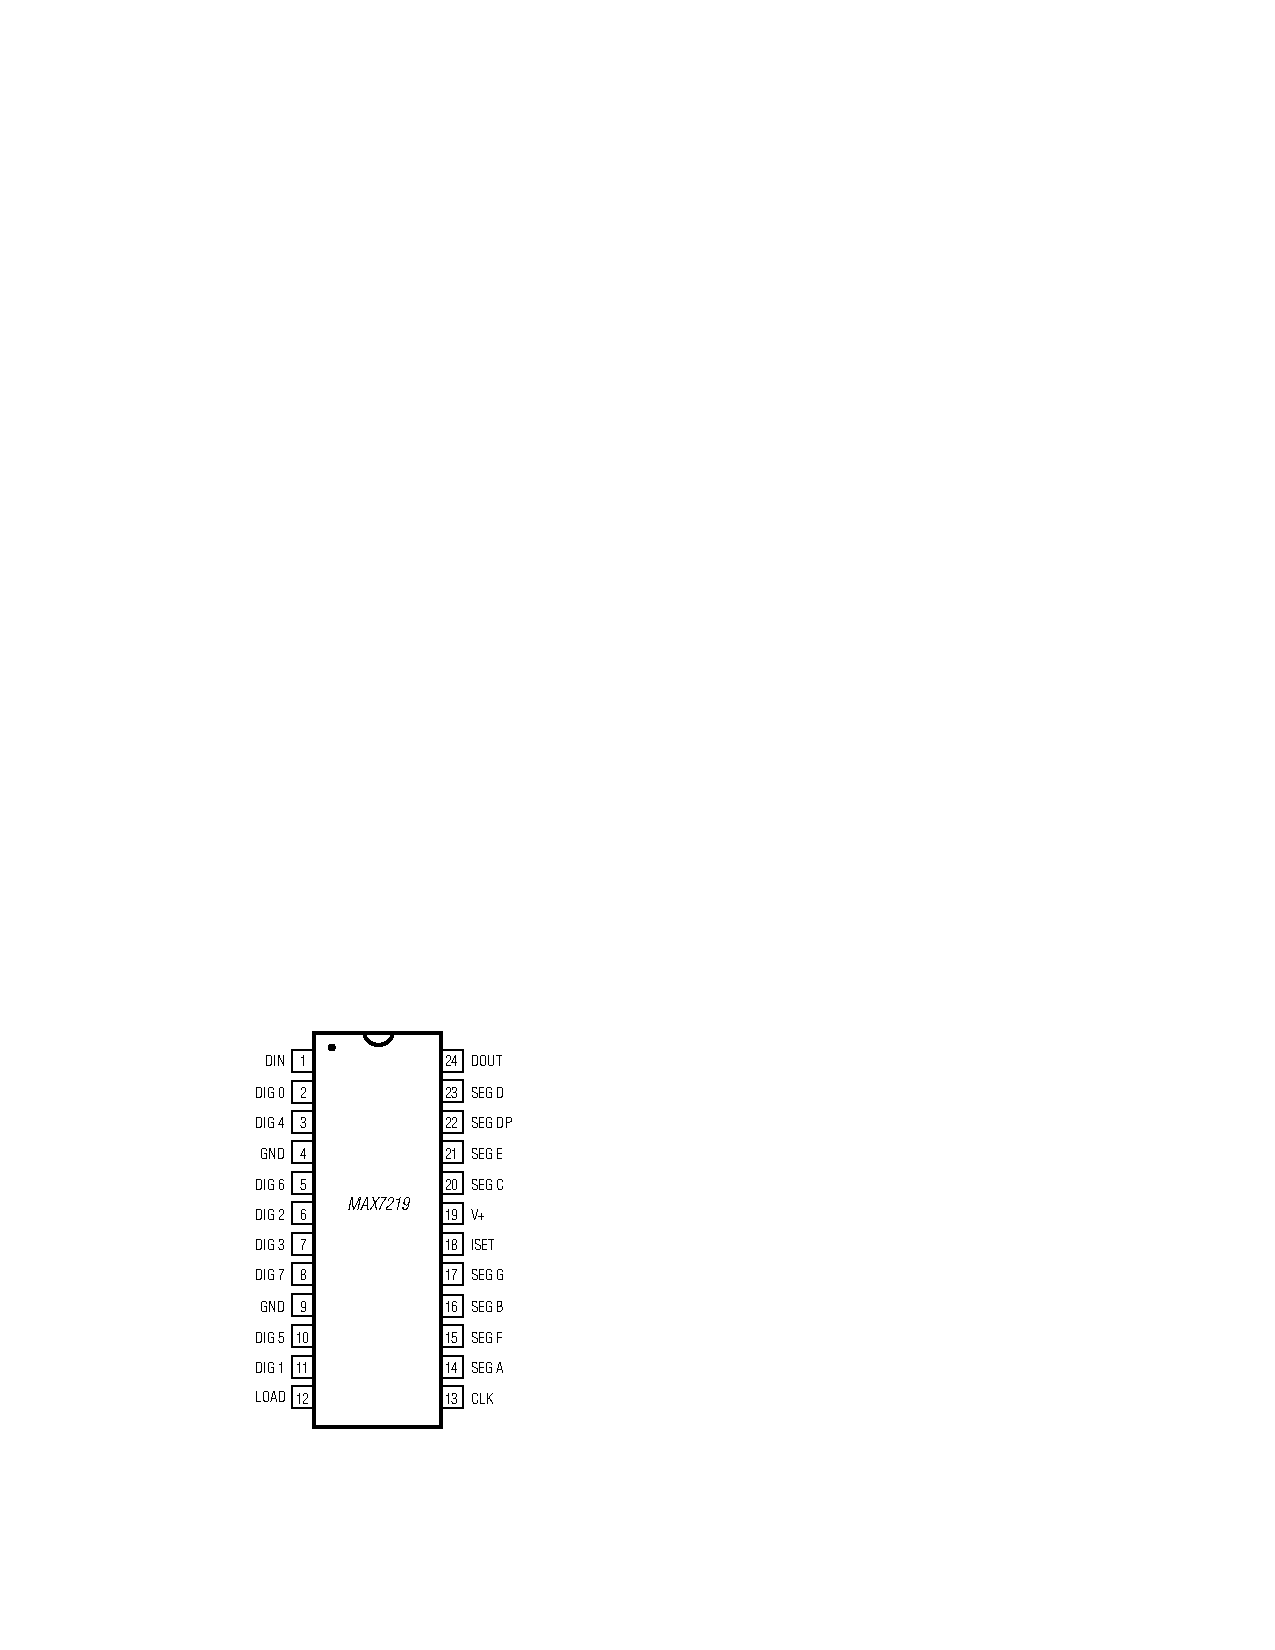
\includegraphics[scale=1.2]{imagenes/hw/max.pdf}
	 \caption{Configuración de pines del chip MAX7219.}
	  \label{fig:MAX-pines}
	\end{center}
\end{figure}

\begin{table}[htp!]
\centering
\caption{Descripción de los pines del MAX7219}
\label{table:MAX-pines}
\begin{tabular}{C{10mm} C{14mm} L{108mm}}
\hline
Pin               & Nombre          & Función    \\ \hline
1                 & DIN             & Pin de datos seriales. Los datos son cargados en el registro de 16 bits en cada flanco ascendente del clock. \\
2, 3, 5–8, 10, 11 & DIG 0 - DIG 7    & Líneas de transmisión de ocho dígitos que absorben corriente del cátodo común de la pantalla. El MAX7219 deja en V+ cuando esta apagado. Los dígitos están en alta impedancia cunado se apaga.\\
4, 9              & GND             & Tierra.\\
12                & LOAD            & Pin de control. Los últimos 16 bits del Serial Data son cargados en el flanco ascendente. \\
13                & CLK             & Pin de clock serial. En cada flanco ascendente, los datos sin shifteados dentro de un registro interno. En cada flanco descendente los datos salen de DOUT. En el MAX7221, la entrada CLK está activa solo mientras LOAD está baja. \\
14–17, 20-23      & SEG A–SEG G, DP & Las unidades de siete segmentos y el punto decimal impulsan la fuente de corriente a la pantalla. Cuando un controlador de segmento está apagado, se conecta a GND.\\
18                & ISET            & Conectar a  $V_{DD}$ a través de una resistencia ($R_{SET}$) para configurar la corriente que pueda entregar a los dígitos y segmentos. \\
19                & V+              & Fuente positiva de corriente, conectar a 5 V. \\
24                & DOUT            & Salida de datos en serie. Los datos en DIN son válidos en DOUT 16.5 ciclos de reloj más tarde. \\ \hline
\end{tabular}
\end{table}

El MAX7219, como se mencionó anteriormente, interpreta comandos de 16 bits. El byte mas significativo de esta palabra de 16 bits codifica el registro que se modificará con el comando. Hay 16 registros con lo cual cuatro bits de este byte se utilizan para direccionar a ellos. Se puede ver en la tabla \ref{tab:max-cmdaddr} parte del formato de un comando, específicamente la dedicada al direccionamiento del registro. Se puede ver también en mejor detalle el formato del contenido de cada comando (el byte menos significativo) en el datasheet del MAX7219 \cite{MAX7219}.
\begin{table}[ht!]
	\centering
	\caption{Mapa de direccionamiento de registros del MAX7219.}
	\vspace{0.2cm}
	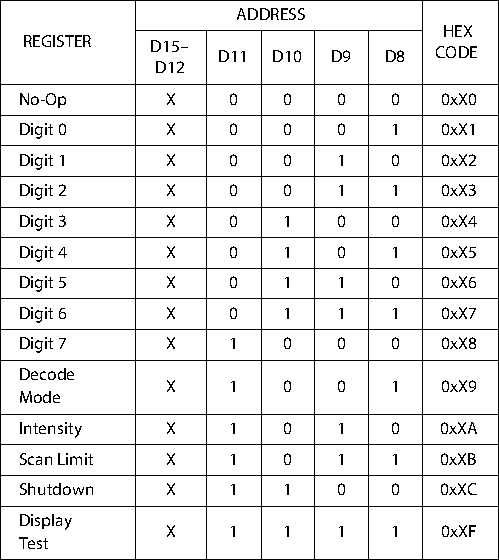
\includegraphics[scale=1]{imagenes/max-cmdaddr.pdf}
	\label{tab:max-cmdaddr}
\end{table}

\subsubsection{Matriz de LEDs} \label{sec:matriz-leds}
La matriz está formada por 64 LEDs organizados en ocho filas y ocho columnas.

Tener control independiente sobre cada LED sería prohibitivamente complicado. Por esto, cada LED se conecta de la siguiente manera: cada LED $L_{i j}$ (donde el subíndice $i$ representa la fila y $j$ la columna, $i=1, 2, ..., 8$, $j = 1,2, ..., 8$), tiene su ánodo conectado a un nodo circuital $C_j$ y su cátodo conectado a un nodo circuital $F_i$. Cada $C_j$ está conectado a DIGj y cada $F_i$ está conectado a SEGi. Este conexionado se puede ver en la figura \ref{fig:modulo-led}.

\begin{figure}[ht!]
	\centering
	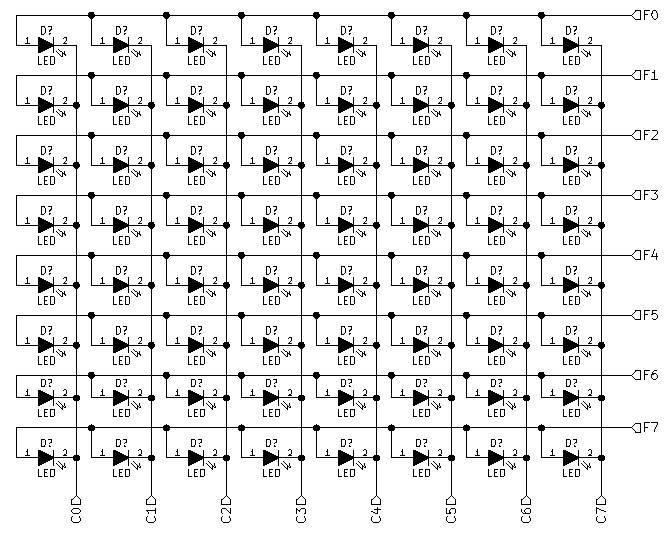
\includegraphics[width=0.7\linewidth]{imagenes/hw/modulo-led.pdf}
	\caption{Esquema de conexiones de la matriz de LEDs.}
	\label{fig:modulo-led}
\end{figure}

La manera que se obtiene la ilusión de tener control independiente sobre cada led se logra explotando el efecto estroboscópico: el MAX7219 mantiene normalmente los nodos $C_j, j = 1, 2, ... ,8$ en alto. Para mostrar una imagen, pone primero pone $C_1$ en bajo y a la vez pone en alto en o en bajo los $S_i, i=1,2,...,8$ para que, por un período corto de tiempo, queden alumbrados los LEDs como correspondan. Luego se procede a hacer lo mismo con $C_2$, hasta llegar a $C_8$ y repetir indefinidamente el procedimiento. Esto se hace a una frecuencia que resulta imperceptible al ojo humano y no se puede apreciar \emph{flicker}.

Se analizaron las dimensiones más apropiadas para la utilidad del cartel y se llegó a una separación de 12mm entre LEDs la cual mantiene un dpi apropiado (consiguiendo verse las letras a una distancia aproximada de 10 metros). 
Todas las medidas estimativas pueden observarse con mayor detalle en la figura \ref{fig:modulo-led-dimensiones}.

\begin{figure}[ht!]
	\centering
	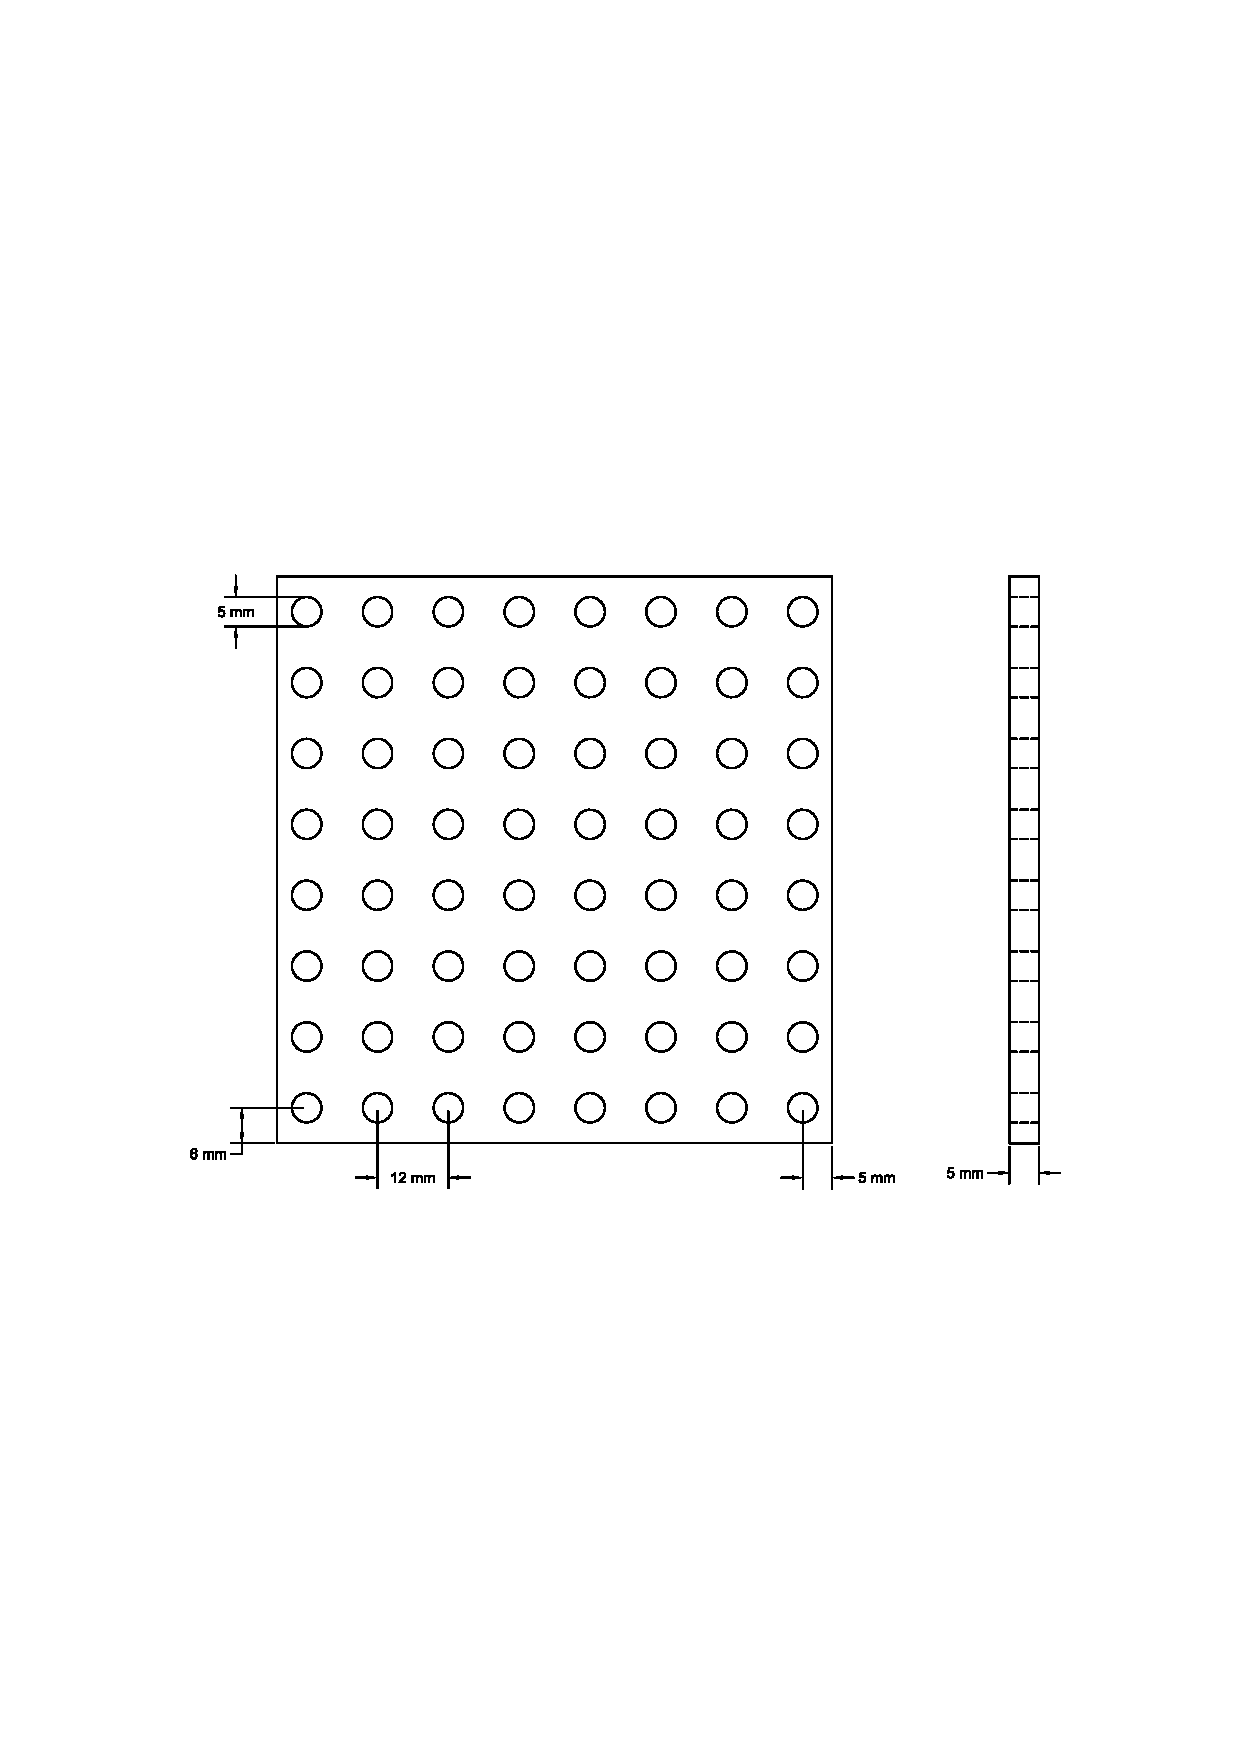
\includegraphics[width=0.8\linewidth]{imagenes/hw/modulo-led-dimensiones.pdf}
	\caption{Dimensiones de la matriz de LEDs.}
	\label{fig:modulo-led-dimensiones}
\end{figure}

Cada uno de los MAX7219 está conectado a una matriz, sus conexiones se pueden observar en el diagrama \ref{fig:MAX-matriz}. Adicionalmente, en la figura \ref{fig:MAX-matriz-real} se observa el prototipo que complementa el esquema de conexión de la figura previamente mencionada.

A la hora de efectuar las conexiones, se debe prestar principal atención a la orientación de la matriz. En la figura \ref{fig:MAX-matriz-real} se indica claramente cuáles son las filas (y su orden) y cuáles son las columnas. Con dicha información el proceso de conexionado se simplifica.

\begin{figure}[ht!]
	\centering
	\begin{center}
		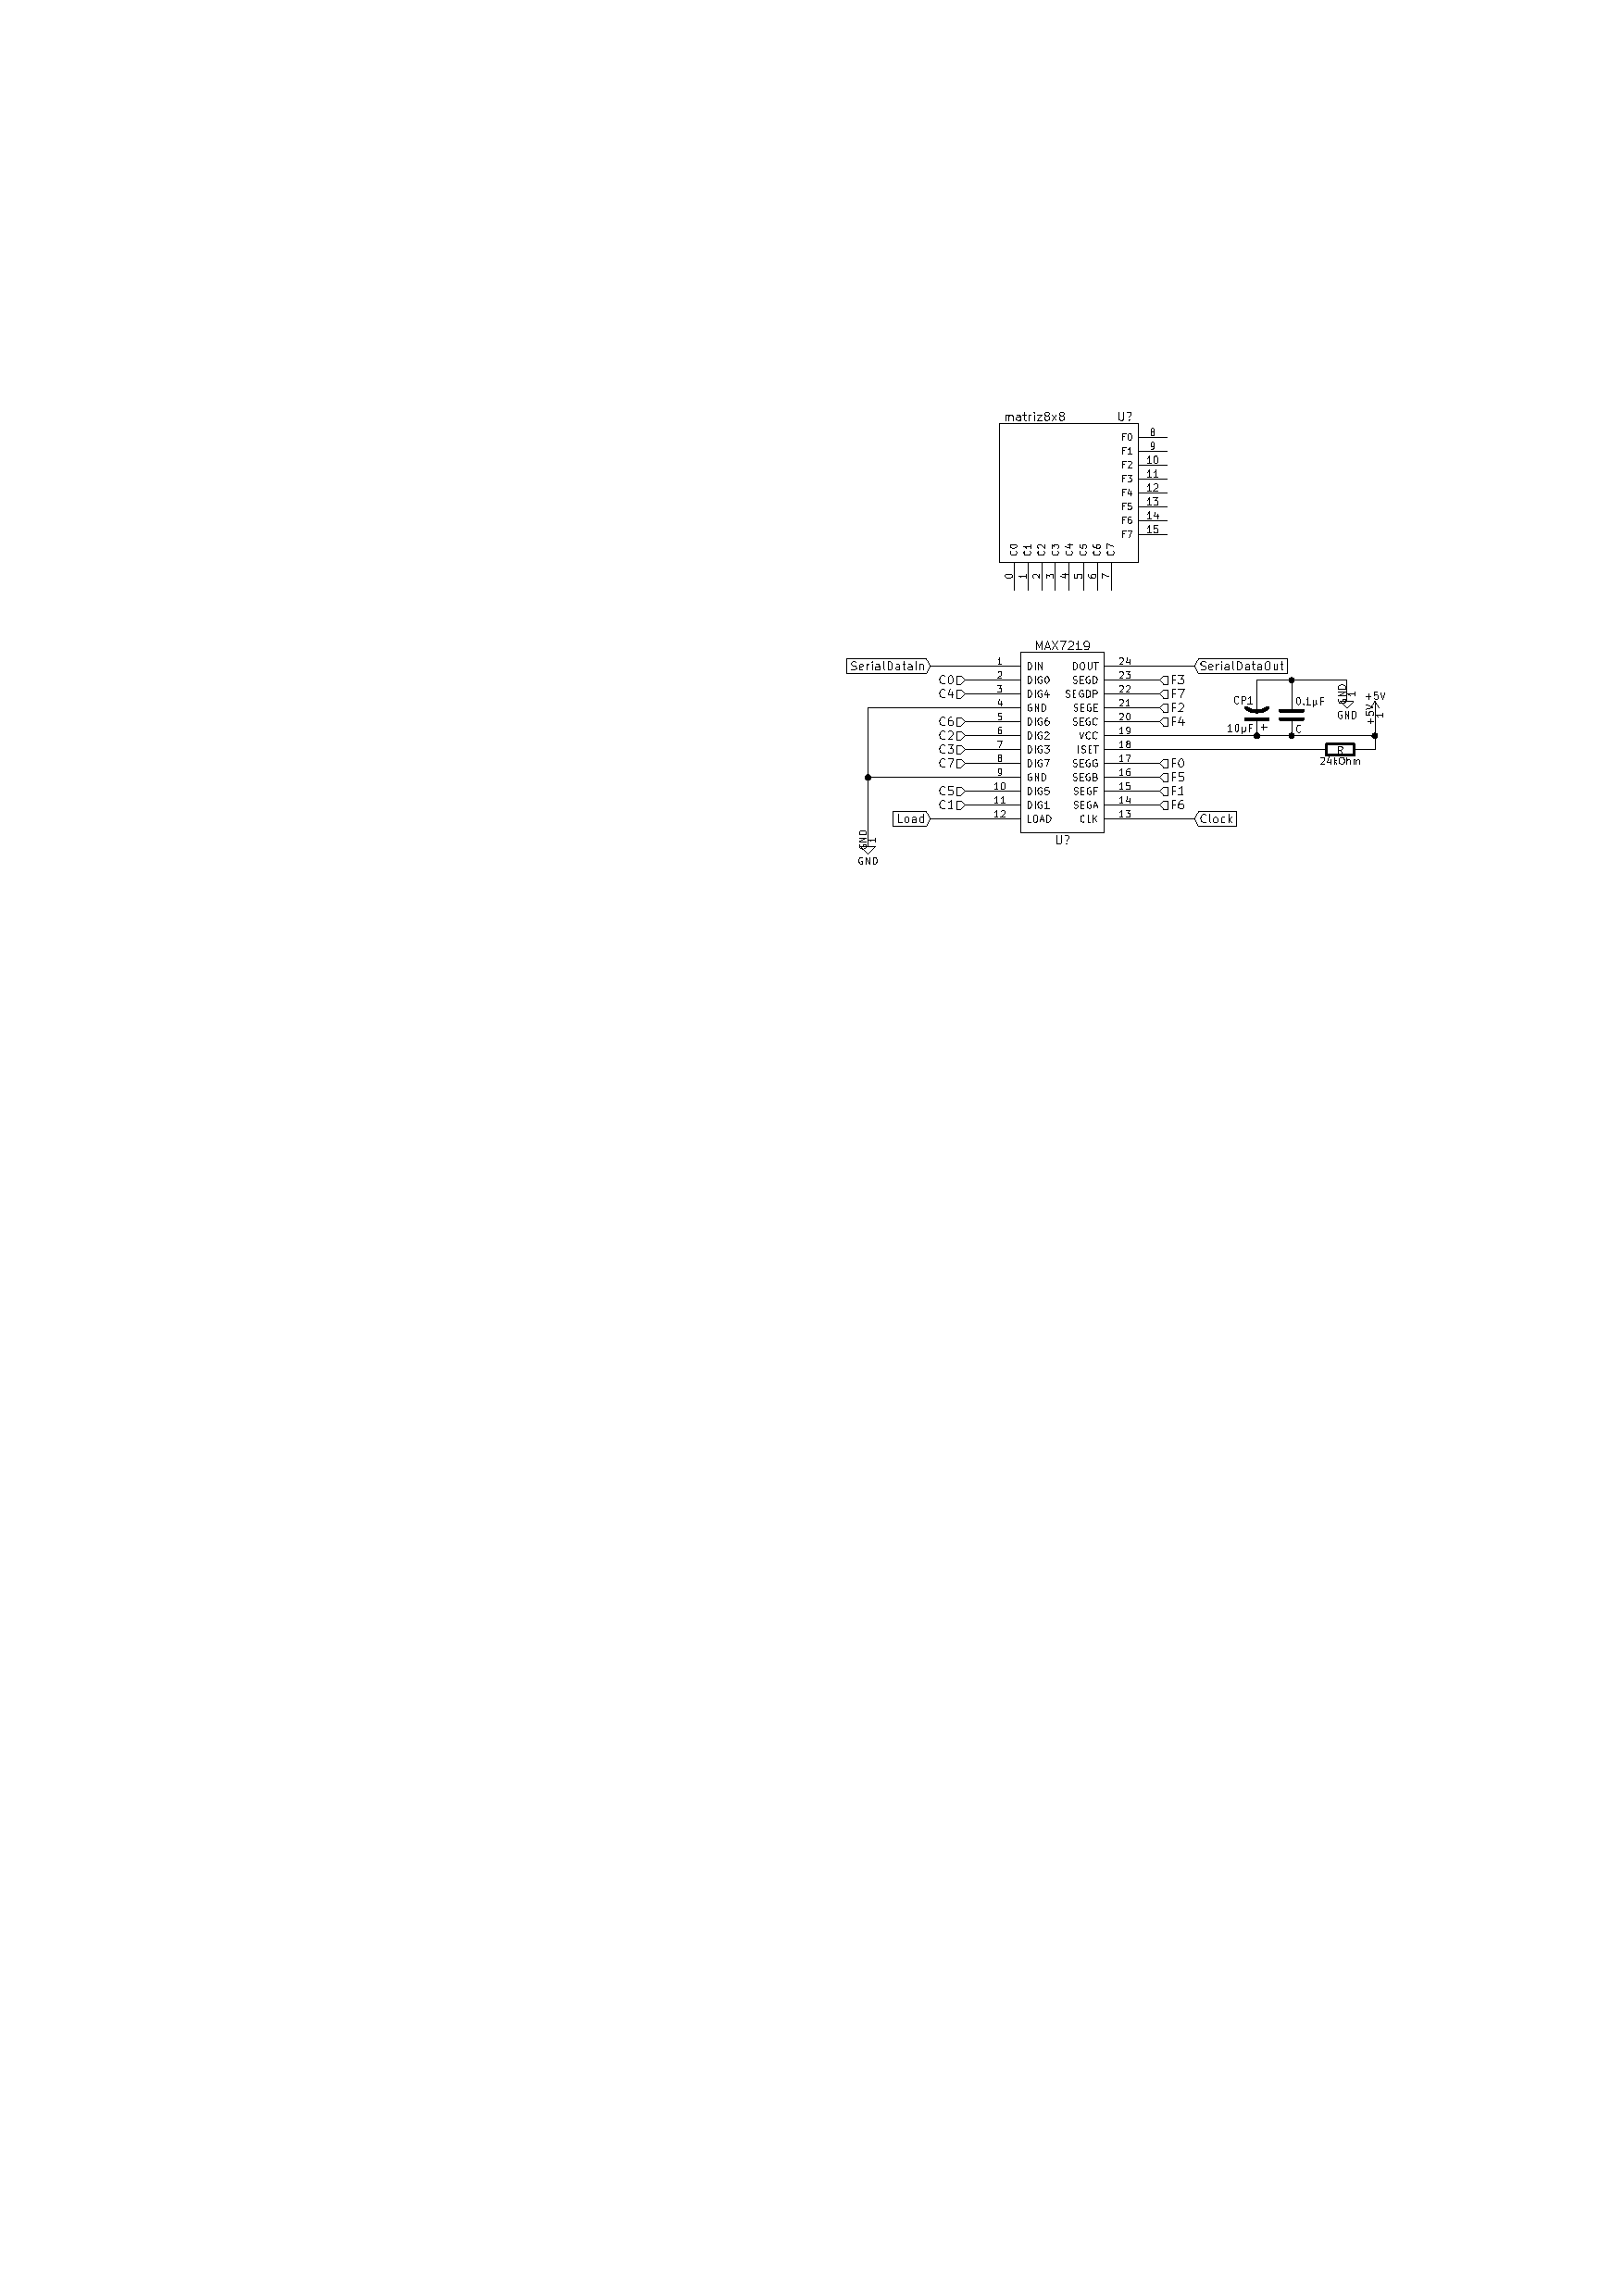
\includegraphics[width=0.8\textwidth]{imagenes/hw/conexion-MAX-matriz.pdf}
		\caption{Conexión entre MAX7219 y su módulo de LEDs.}
		\label{fig:MAX-matriz}
	\end{center}
\end{figure}

\begin{figure}[ht!]
	\centering
	\begin{center}
		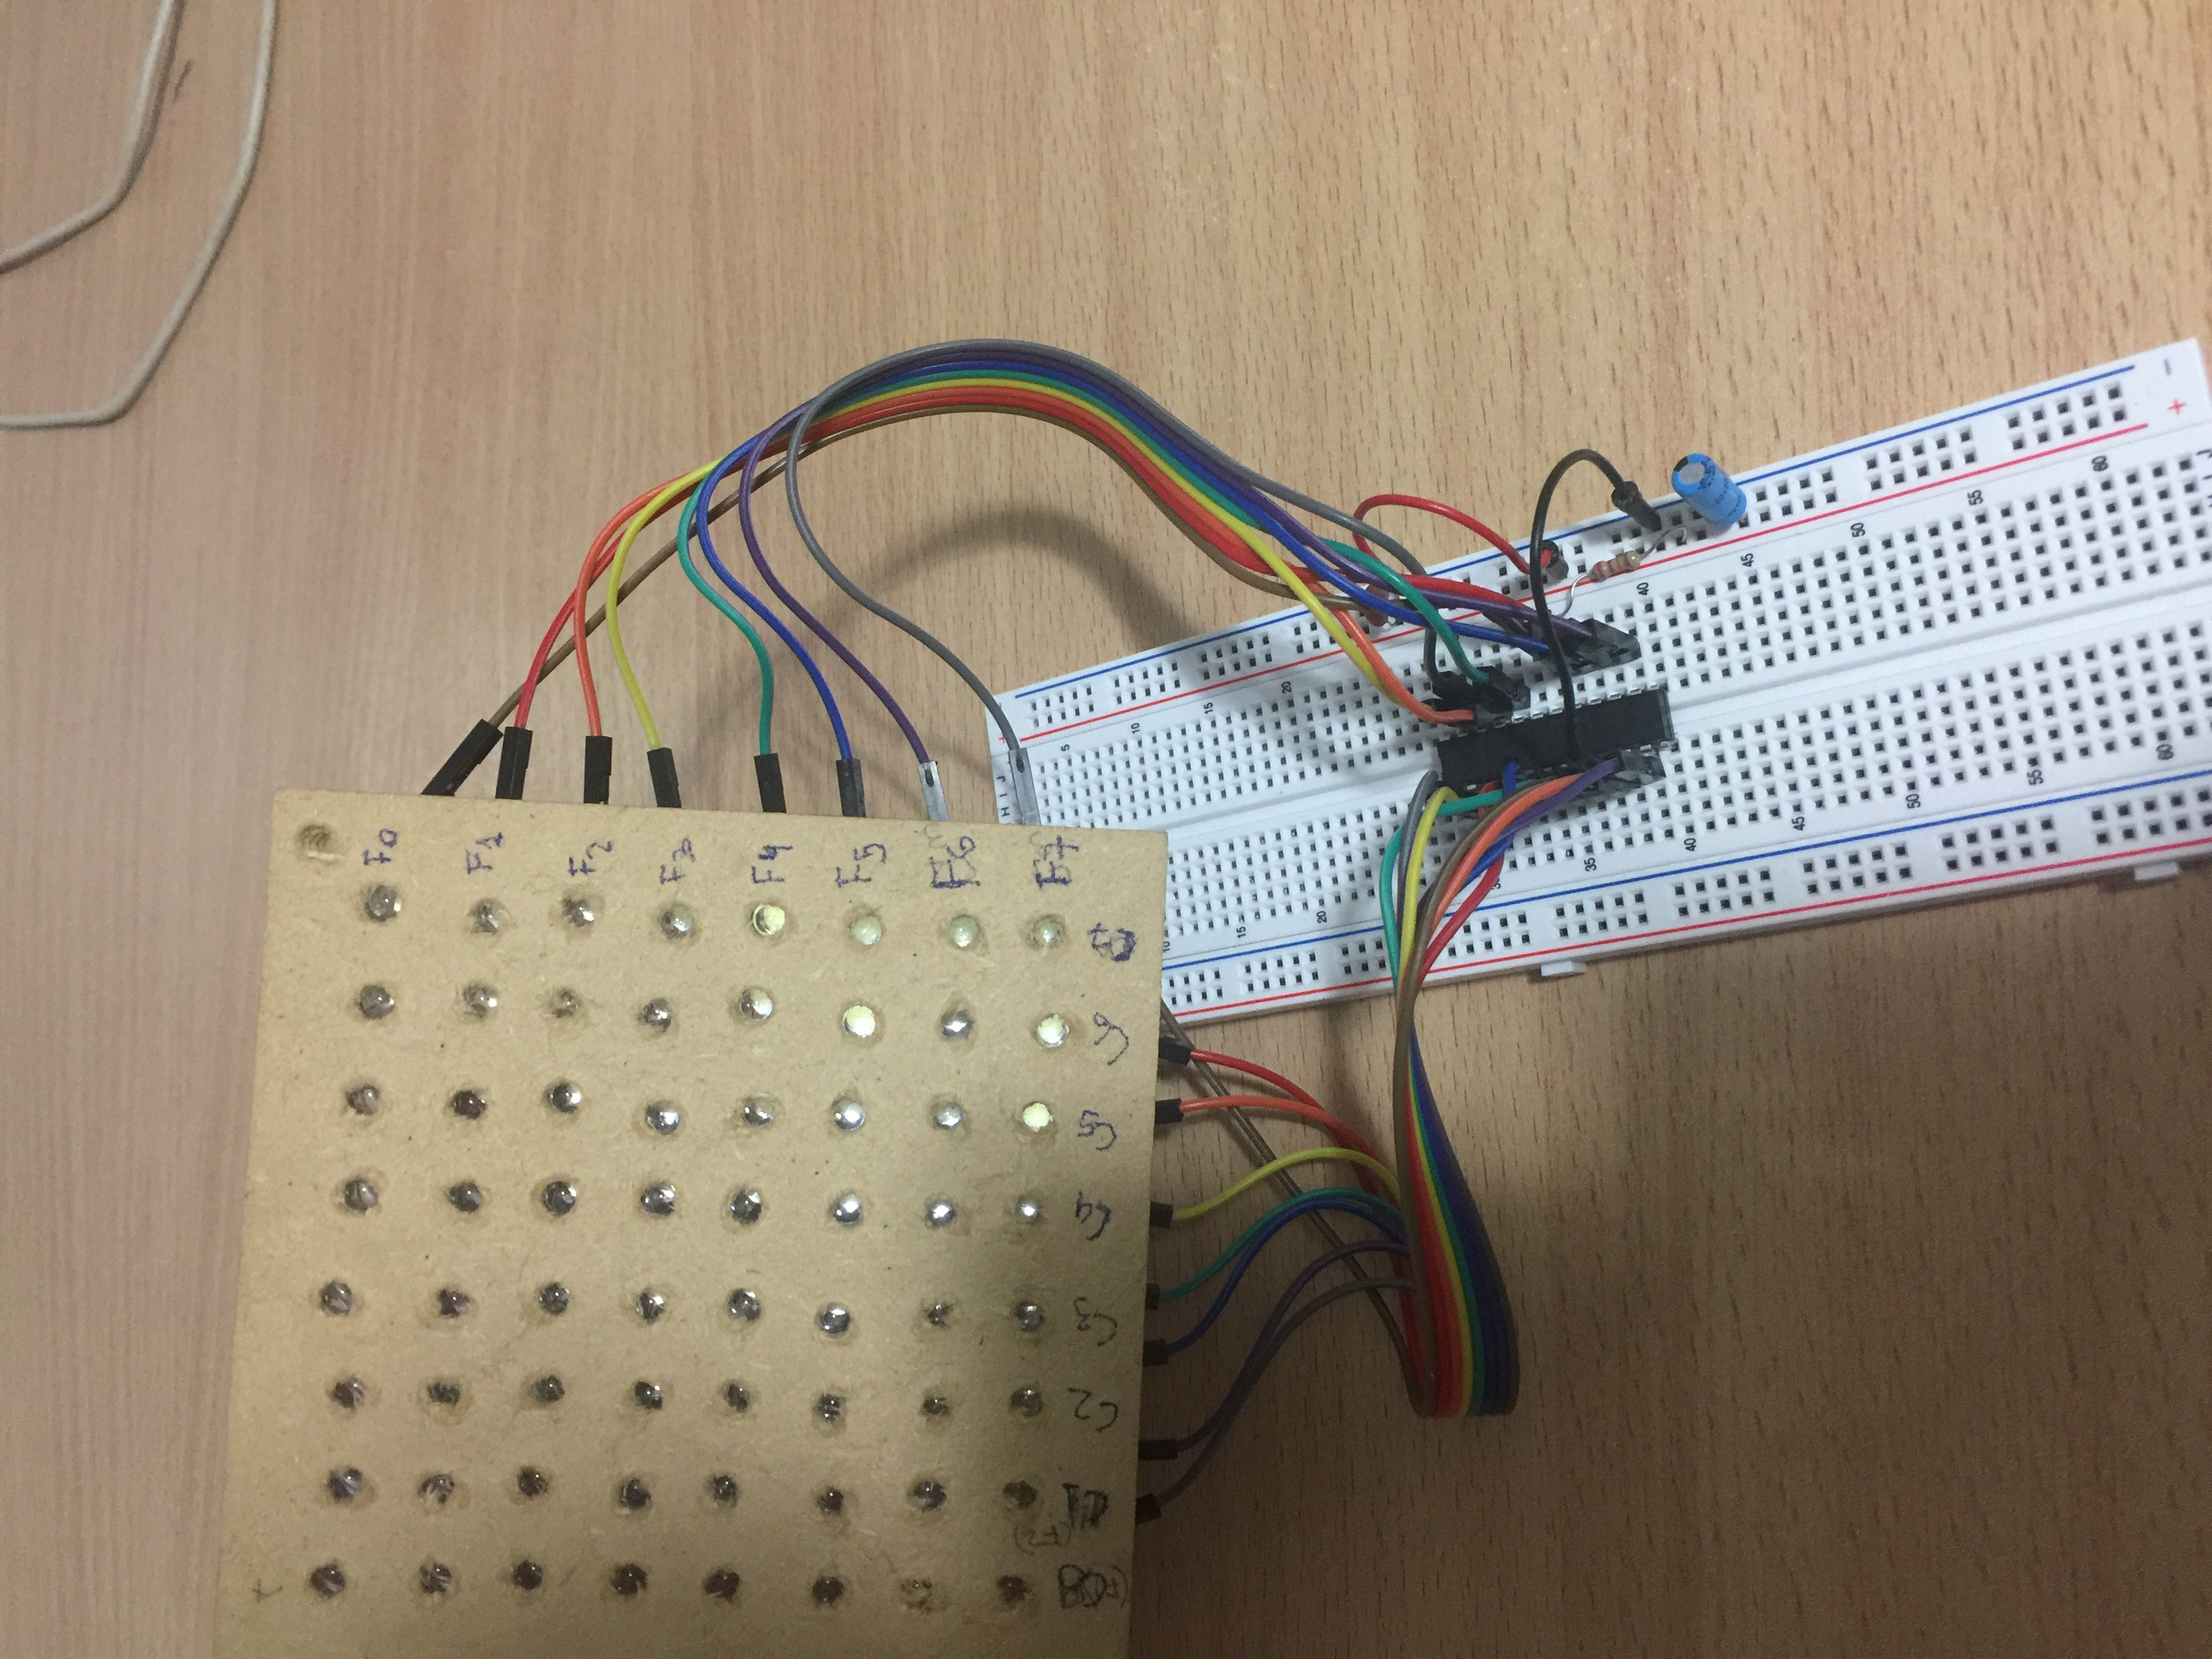
\includegraphics[width=0.8\textwidth]{imagenes/hw/conexion-MAX-matriz.JPG}
		\caption{Fotografía de conexión entre MAX7219 y su módulo de LEDs.}
		\label{fig:MAX-matriz-real}
	\end{center}
\end{figure}


\subsection{Comunicación entre los módulos} \label{sec:comunicacion-modulos}
Para la comunicación maestro-esclavo y esclavo-esclavo se utiliza un protocolo serie de un bit sincrónico. Cada módulo esclavo tiene en su MAX7219 una entrada de serie junto a un clock, de manera que se toma el valor del bit en el flanco ascendente del reloj. A su vez, cada MAX7219 tiene un registro de desplazamiento de 16 bits, que en cada flanco ascendente del clock inserta en orden FIFO al registro un bit (DIN) y, en el flanco descendente del reloj, coloca en su salida el valor del bit más viejo en el registro de desplazamiento (DOUT). Por último, el MAX7219 tiene una entrada llamada LATCH que al pasar a alto, provoca que el MAX7219 \enquote{tome} la palabra de 16 bits, interpretándola como se describió en la sección \ref{sec:max7219}.

De esta manera es posible dirigir una palabra arbitraria a cualquier esclavo, y es particularmente eficiente en el caso en que se debe mandar una palabra a cada MAX7219 y se desea que todas la interpreten a la vez. Es cuestión de simplemente transmitir los datos dirigidos a cada esclavo, uno tras otro, hasta llenar todos los registros de desplazamiento y levantar LATCH. Alternativamente, si se quisiera mandar un sólo comando a un esclavo en particular, basta con insertar \enquote{burbujas} (comandos que no realizan ninguna operación) en la secuencia de bits.

Es posible expandir el cartel con $N$ esclavos. En la figura \ref{fig:MAX-MAX} se observa la forma en que se debe realizar la interconexión de los dispositivos integrados.

\begin{figure}[ht!]
	\centering
	\begin{center}
		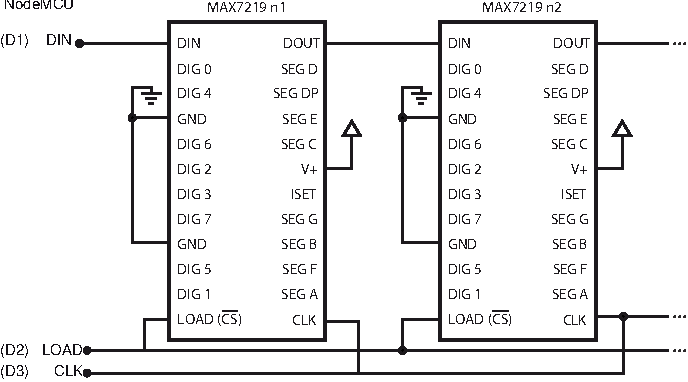
\includegraphics[width=\textwidth]{imagenes/hw/MAX-daisychain.pdf}
		\caption{Conexión entre dos MAX7219.}
		\label{fig:MAX-MAX}
	\end{center}
\end{figure}

El procedimiento que se realiza para cargar los mapas de bits en cada esclavo consiste en transmitir a cada MAX7219 los LEDs que debe encender y apagar en cada columna. Para ello debe enviar palabras de 16 bits por serie. Es decir, primero envía la información de la columna 1, después la 2, y así hasta la 8.

\begin{table}[ht!]
	\centering
	\caption{Formato de la palabra de comando del MAX7219.}
	\label{table:trama-spi}
	\begin{adjustbox}{max width=\textwidth}
	\begin{tabular}{|c|c|c|c|c|c|c|c|c|c|c|c|c|c|c|c|}
	\hline
	D15 & D14 & D13 & D12 & D11   & D10   & D9   & D8   & D7 & D6 & D5 & D4 & D3 & D2 & D1 & D0 \\ \hline
	X   & X   & X   & X   & \multicolumn{4}{c|}{ADDRESS} & \multicolumn{1}{c}{ MSB } & \multicolumn{6}{c}{ DATA } & \multicolumn{1}{c|}{ LSB } \\ \hline
	\end{tabular}
	\end{adjustbox}
\end{table}

Para realizar este proceso, la figura \ref{fig:spi-timing-diagram} muestra un diagrama a lo largo del tiempo de la forma de enviar cada bit. En ella se puede observar que el primer paso consiste en bajar la señal de LOAD y esperar un instante de tiempo (aproximadamente un microsegundo).
Luego se genera una señal de CLK de onda cuadrada y de frecuencia de a lo sumo 1Mhz con ciclo de trabajo de $50 \%$. No es necesario que CLK sea una señal periódica, es suficiente que se respeten los tiempos de setup y hold, llevando CLK a alto luego de haber transcurrido $t_{DS}$ con el dato ya en DIN y mantenerlo por $t_{DH}$.

% Cuando finaliza el envío de los 16 bits, se debe subir la señal de LATCH. En ese momento, el MAX7219 almacena, en sus registros internos, el comando recibido. Todos los comandos son de dos bytes, sin embargo, se puede enviar más de esa cantidad. Esta funcionalidad se utiliza para enviar instrucciones a los demás MAX7219 que están conectados en serie. Lo que ocurre es que la información se recibe en el flanco ascendente de CLK y se envía, hacia el siguiente chip, por el pin DATAOUT en el flanco descendente. De esta forma, en una iteración se pueden configurar una columna de cada módulo de 8x8 LEDs.

\begin{figure}[ht!]
	\centering
	\begin{center}
		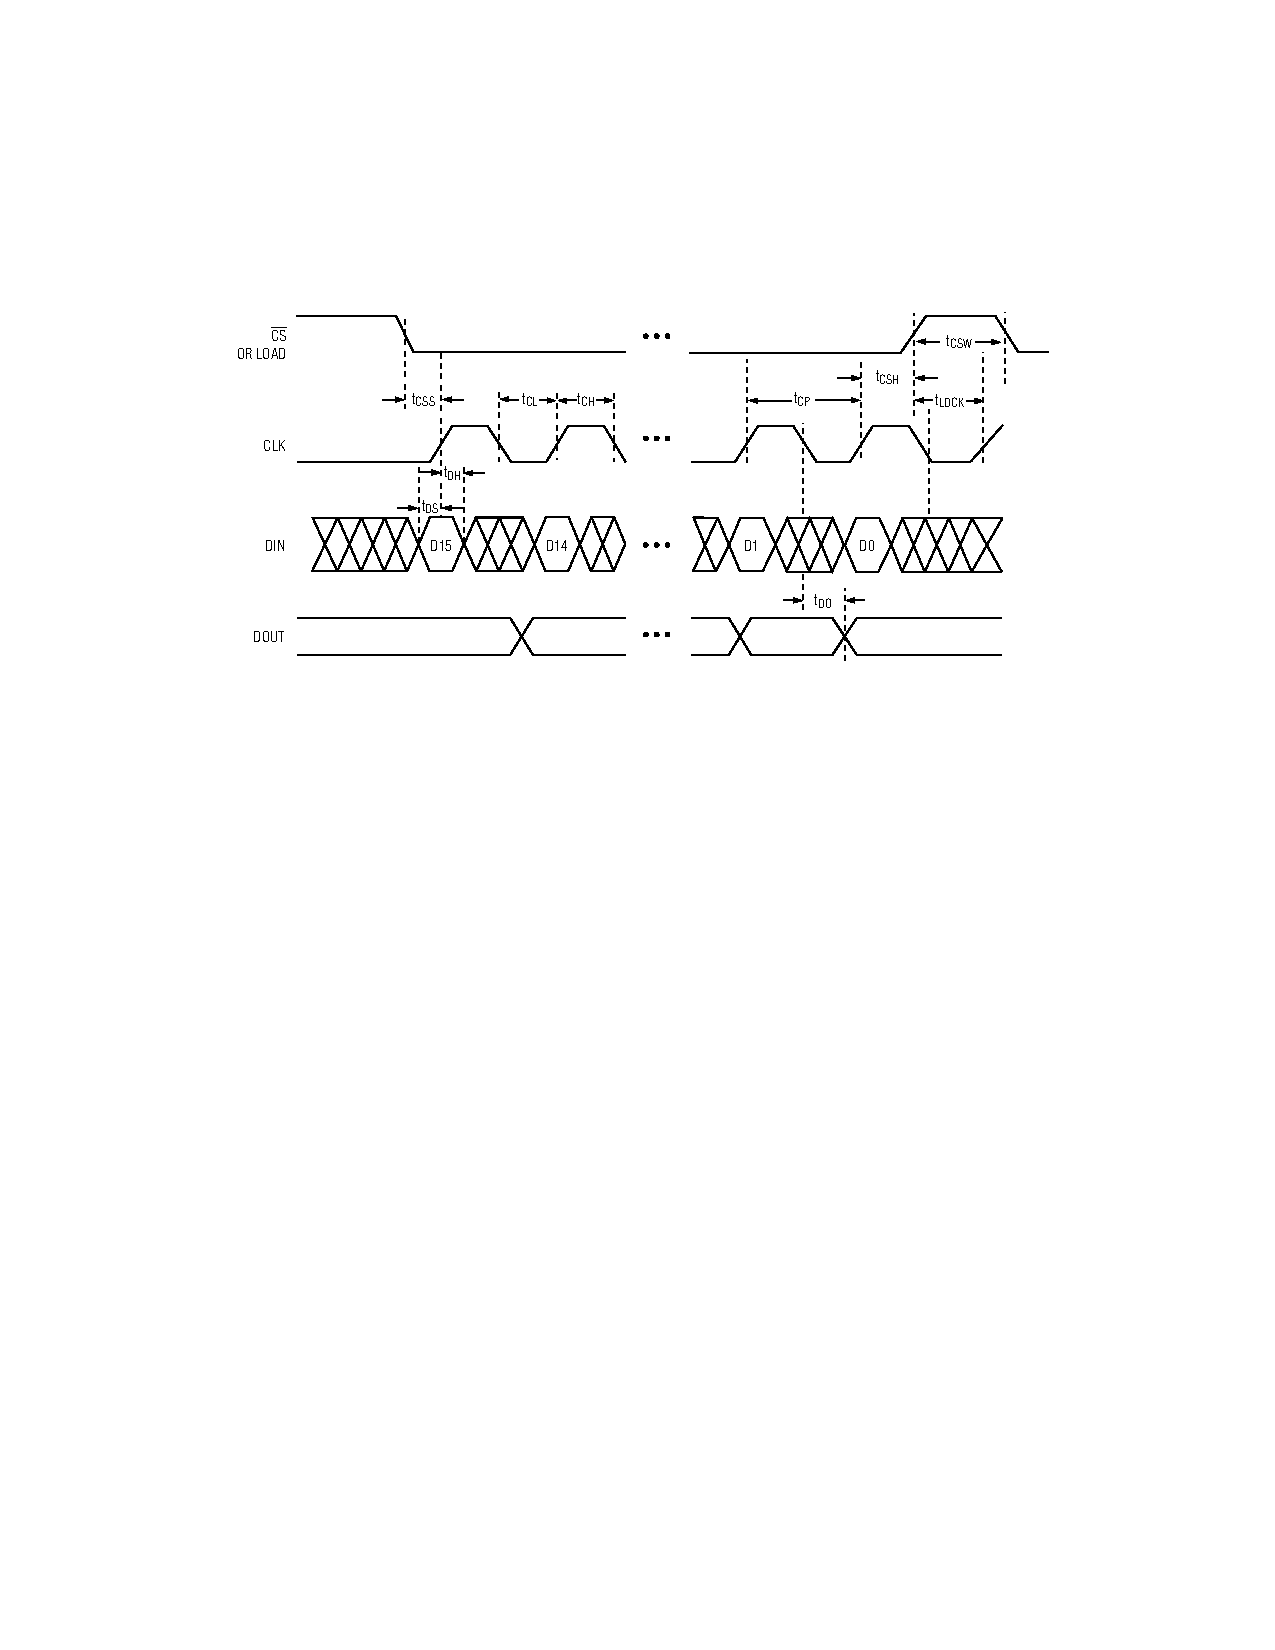
\includegraphics[width=\textwidth]{imagenes/hw/timingDiagram.pdf}
		\caption{Diagrama de tiempo de las señales del MAX7219.}
		\label{fig:spi-timing-diagram}
	\end{center}
\end{figure}

\subsubsection{Diseño de PCB}
Los componentes implicados en el sistema del módulo esclavo cumplen una función relativamente pasiva. El mensaje programado en el master se transmitirá al esclavo de la manera especificada en la sección \ref{sec:max7219}.

Los LEDs cumplirán la función de visualizar el espacio correspondiente a un caracter del mensaje transmitido. El PCB contendrá las pistas que cerrarán el circuito electrónico del módulo.

El MAX7219 leerá las señales de datos del mensaje e indicará a cada fila y columna qué LEDs deben estar encendidos en cada instante, teniendo en cuenta el retardo necesario para que los subsiguientes módulos puedan visualizar la parte que les corresponda del mensaje de tal manera que en conjunto éste pueda ser leído uniformemente y con un desplazamiento homogeneo en toda la cadena de módulos esclavo. El MAX7219 también se encargara de, dejando pasar el retardo necesario, pasar el mensaje al siguiente módulo para el procesamiento de la parte que corresponda más adelante.

Los capacitores y la resistencia cumplen funciones pasivas.

Los conectores hembra de 8 pines permitirán la conexión con las filas y las columnas de la matriz respectivamente.

Los conectores macho de 5 pines permitirán la interconexión con otros esclavos o bien con el maestro para la transmisión de las 3 señales de datos y las 2 de alimentación.

Se puede ver en la figura \ref{fig:pcb-slave} el diseño final de la PCB del esclavo.

\begin{figure}[ht!]
	\centering
 	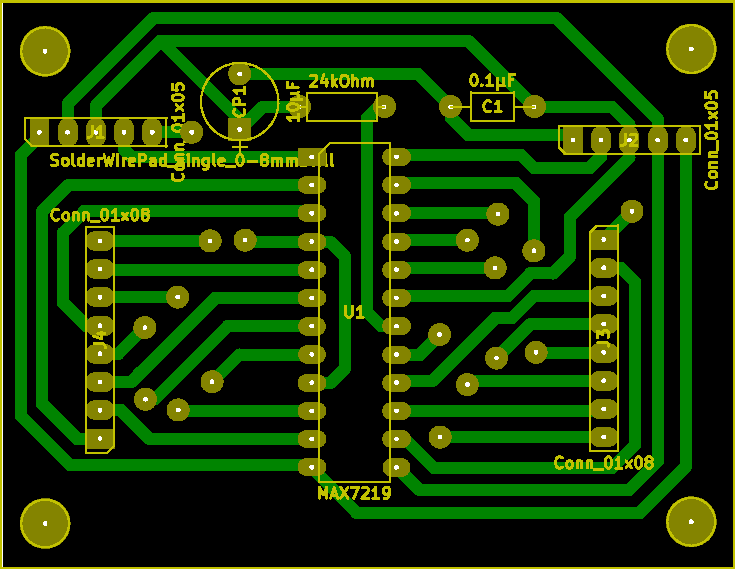
\includegraphics[width=\linewidth]{imagenes/pcb-slave.pdf}
	\caption{PCB del módulo esclavo.}
	\label{fig:pcb-slave}
\end{figure}

\clearpage
\section{Software}\label{sec:sw}
El software del sistema está formado por dos componentes. En primer lugar se encuentra el firmware que corre sobre el controlador del cartel y por otro lado, la aplicación de PC que corre sobre una computadora de escritorio o notebook.

El cartel será alcanzable por la PC a través de una red IP. Esto significa que no es estrictamente necesario que la PC y el cartel estén en una misma red física, sino que basta con que exista una ruta entre ellos. Sin embargo, el cartel está asociado a la red estrictamente mediante 802.11 (WiFi), mientras que la PC puede tener conectividad al cartel mediante diversas formas. Detalles básicos sobre el Internet Protocol y mecanismos de routeo no se discutirán en este informe.

\subsection{Interacción PC-Cartel}
La comunicación que se da entre la PC y el cartel sigue el modelo de Cliente-Servidor donde la PC es el cliente mientras que el cartel cumple el rol de servidor. Esto significa que es la PC quien comienza a interactuar con el cartel, estableciéndose un circuito virtual que permanecerá activo durante un cambio de mensaje o configuración en el cartel, o incluso cuando se quiera recuperar el mensaje que se está mostrando actualmente.

Adicionalmente, la aplicación de PC puede pedirle al sistema, las credenciales de red a las que el microcontrolador del cartel se encuentra conectado. Esta operación, al igual que las mencionadas anteriormente, forman parte de las funcionalidades del sistema.

El tiempo que permanece activa la conexión debe ser, lo más corto posible. El cartel debe cerrar una conexión que permanezca ociosa por más de un tiempo configurable.

La razón de ésto se debe a que un individuo malintencionado podría iniciar una conexión hacia el cartel y no mandar ningún mensaje, efectivamente bloqueando el uso legítimo del cartel.

Cabe recordar que por limitaciones técnicas del SDK utilizado, el controlador del cartel sólo puede aceptar una conexión de este tipo\footnote{Una conexión cifrada con TLS} a la vez. 

Resulta necesario, entonces, elegir un tiempo (a partir de ahora, denominado tiempo de timeout) lo suficientemente corto para que esta medida sea efectiva. Sin embargo, no puede ser tan corto de forma que descarte conexiones que legítimamente tienen un retardo (por ejemplo, por congestión de la red).  Este tiempo es una constante ajustable en el código del firmware del cartel.

La comunicación entre la PC y el cartel es bidireccional, debido a que hay determinados comandos que requieren una respuesta por parte del microcontrolador, como por ejemplo información respecto al mensaje actual o las credenciales de red.
Mientras que otras respuestas, son solo para indicar si la operación enviada se resolvió correctamente o no.

Es por este motivo, que resulta necesario implementar un protocolo de comunicación de red, que permita el intercambio de información con sentido, entre los dos módulos de sw.
Este protocolo se encuentra detallado en la sección \ref{sec:protocolo} y su diseño e implementación es exclusivo para el presente proyecto.

La figura \ref{fig:petri-net} describe el mecanismo de interacción entre la PC y el cartel mediante una red de Petri. En ella se nombra Servidor (S) al cartel y Cliente (C) a la aplicación de PC. Lo importante a entender es que este mecanismo se basa en turnos; el cliente C envía un pedido y el servidor S devuelve una respuesta. No se pueden transmitir dos pedidos ni dos respuestas seguidas.

\begin{figure}[ht!]
	\centering
	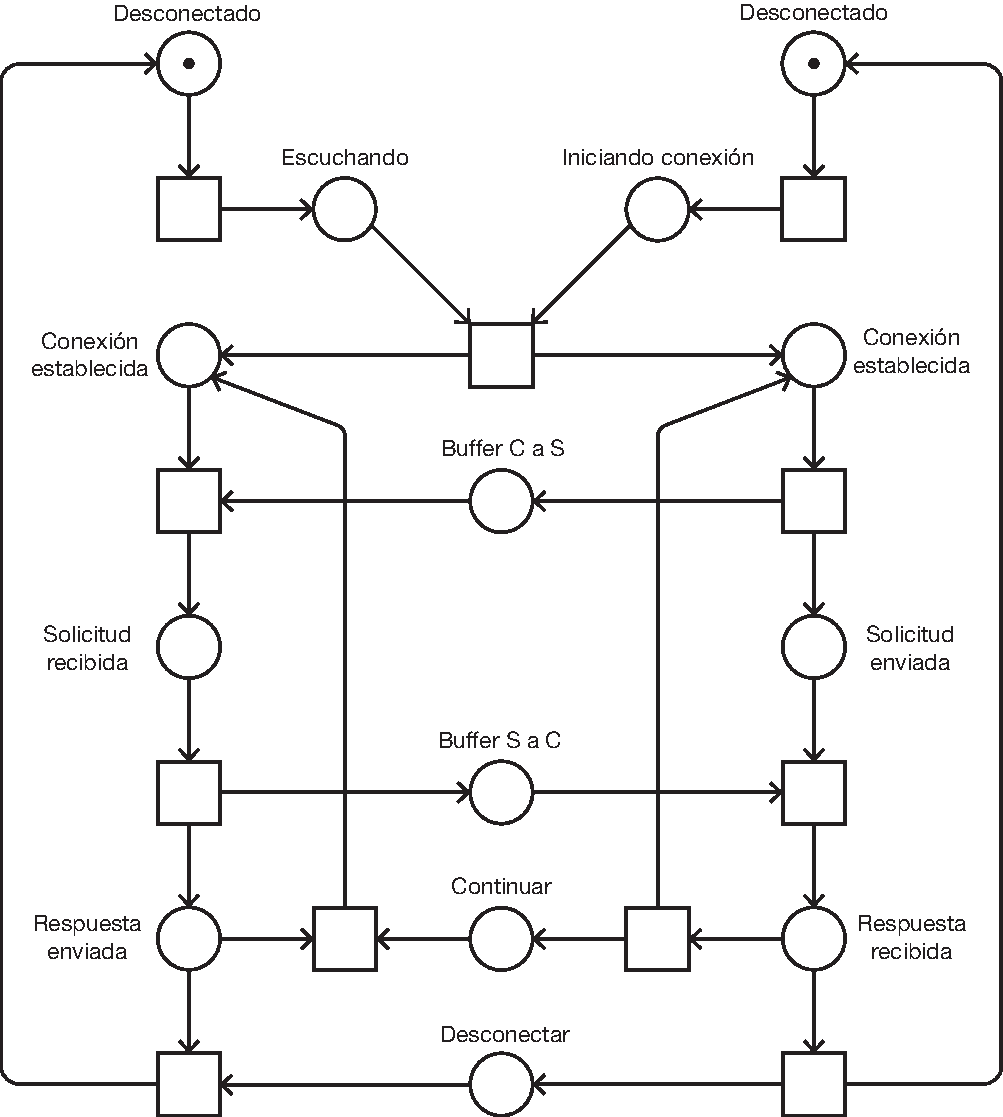
\includegraphics[width=1\linewidth]{imagenes/petri-net.pdf}
	\caption{Red de Petri modelando la interacción entre la aplicación de PC y el cartel.}
	\label{fig:petri-net}
\end{figure}


\subsection{Firmware}
El firmware del controlador del cartel es quien se encarga de aceptar pedidos de la aplicación de PC y ejecutar las acciones de cambio de mensaje, parámetros de animación, configuración WiFi o de contraseña. Además, como se explicó en la sección \ref{sec:hw}, el ESP8266EX envía la configuración de las matrices de LED por serie de manera sincrónico.




\subsubsection{Arquitectura general del programa}

El software que corre en el microcontrolador del cartel debe escuchar conexiones, y una vez establecida una conexión iniciada por la aplicación de PC, debe esperar a recibir un mensaje de autenticación con contraseña antes de permitir cambios del contenido del cartel.

Una vez que el usuario se autentica, el cartel espera un pedido de la aplicación de escritorio. Las interacciones posibles están descritas en mayor detalle en la sección \ref{sec:protocolo}.

El comportamiento del microcontrolador puede describirse como una máquina de estado finita jerárquica, como lo muestra la figura \ref{fig:fsm-micro}.

\begin{figure}[ht!]
	\begin{center}
		\centering
		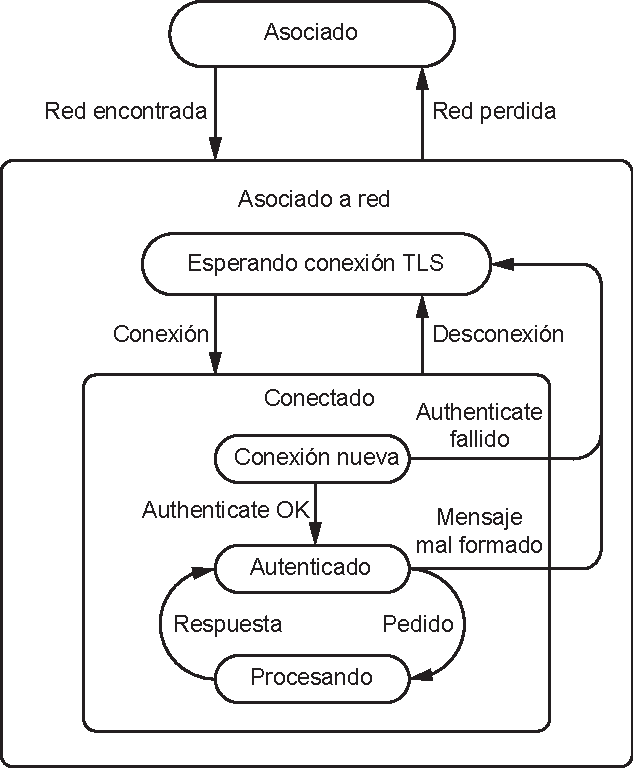
\includegraphics[scale=0.8]{imagenes/fsm-micro.pdf}
		\caption{Máquina de estados finitos jerárquica del manejo de conexión en el microcontrolador.}
		\label{fig:fsm-micro}
	\end{center}
\end{figure}



\subsubsection{Requerimientos generales del programa embebido}

El programa que corre sobre el microcontrolador ESP8266 necesita conectarse a una red WiFi preexistente a fin de poder establecer una comunicación cifrada bajo el protocolo TLS con el cliente.
En esta sección, se hace referencia al cliente como la aplicación de PC.

El software debe actuar como servidor y manejar las peticiones que el cliente realice por medio de la aplicación de PC, detallada en la sección \ref{sec:pc}.
Dichas peticiones se clasifican en dos categorías: del tipo \enquote{get} y del tipo \enquote{get}. Las mismas se explican a continuación.

Las primeras corresponden a pedidos que solicitan información del sistema, mientras que las segundas permiten modificar dicha información.
Dentro de la categoría get, por un lado, el cliente puede loguearse en el sistema, obtener el texto que actualmente se muestra en el cartel, capturar la velocidad con la que se desplaza y con la que parpadea el contenido y pedir la configuración WiFi de la red a la que se encuentra conectado el microcontrolador.

A su vez, el cliente puede cambiar el contenido que desea representar, así como también modificar los parámetros relacionados a la velocidad de desplazamiento y parpadeo del texto.
Adicionalmente es posible modificar la configuración de la red a la que se autenticará la próxima vez que el ESP8266 se reinicie.
Por otra parte, el sistema posee una contraseña que es necesaria para realizar la acción de logueo.
Una vez logueado, dicha clave puede ser modificada. Estas acciones pertenecen a la categoría set.

Respecto de la información de la red, cabe destacar que los posibles parámetros que se pueden solicitar y cambiar son: el SSID, la contraseña WiFi, la dirección IP y la máscara de subred.

La figura \ref{fig:diagrama_casos_de_uso} muestra un diagrama de casos de uso, que describe todas las funcionalidades que el cliente puede realizar.
Adicionalmente, se observa como interactúan dichos pedidos, con el cartel.

\begin{figure}[!ht]
	\centering
	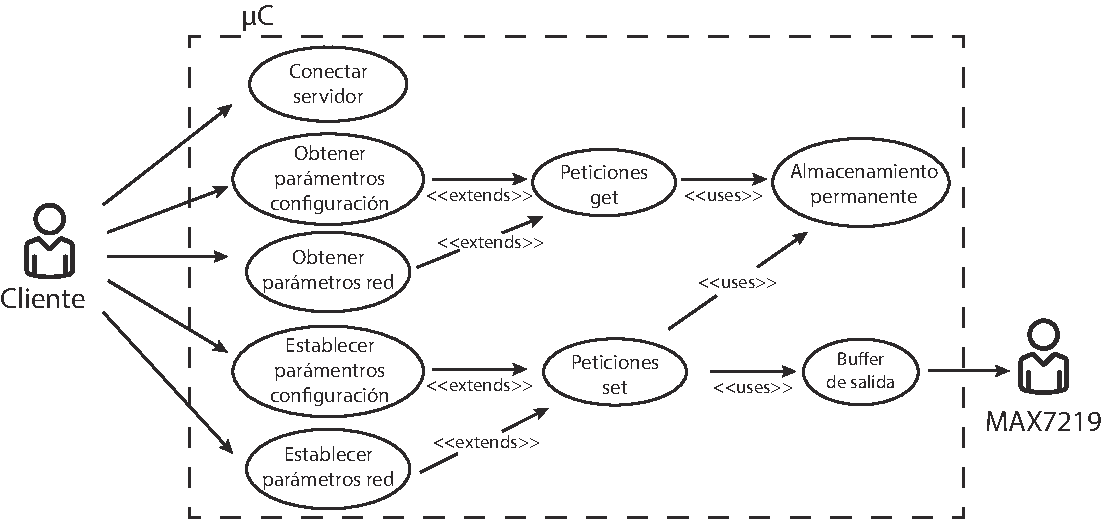
\includegraphics[width=1\linewidth]{imagenes/sistema-caso-de-uso.pdf}
	\caption{Diagrama de casos de usos.}
	\label{fig:diagrama_casos_de_uso}
\end{figure}

En la figura \ref{fig:diagrama_casos_de_uso} se observa, que entre las funcionalidades que el cliente realiza, se encuentra la de modificar los datos del cartel, tal como su contenido, su configuración WiFi y su contraseña del sistema.
Como el sistema puede, eventualmente, ser desprovisto de su alimentación o reseteado, es necesario que dichos cambios persistan aún cuando éstos eventos ocurren.

Por otra parte, el programa debe ser capaz de interpretar los pedidos que realiza el cliente y procesarlos a fin de generar la información que necesita el cartel para encender cada columna de luces.
Es necesario recordar que la matriz de LEDs está compuesta por módulos MAX7219 que son los encargados de recibir los datos enviados por el microcontrolador y encender las columnas de luces según corresponda.



\subsubsection{Secuencia de eventos del lado del microcontrolador}

En esta sección se enuncia brevemente, la secuencia de eventos que el usuario puede realizar con el sistema y cómo el programa responde ante los diferentes pedidos.
Es importante tener presente la figura \ref{fig:diagrama_casos_de_uso} donde se observa el diagrama de casos de uso que describe todas las funcionalidades que el cliente puede efectuar.

En primer lugar, el cartel se conecta a la red WiFi presentando las credenciales previamente almacenadas en la memoria no volátil del microcontrolador.
Esta acción es llevada a cabo gracias a una clase a nivel software denominada WiFiManager.
A su vez, el cliente accede a la aplicación de PC, con el ordenador conectado a la misma red.

El sistema le solicita la contraseña antes de realizar cualquier acción.
Una vez logueado, el cliente puede realizar cualquiera de las funcionalidades previamente enunciadas en la subsección anterior (tanto del tipo get como del tipo set).
Entre las acciones disponibles puede pedir información del texto que actualmente se encuentra representado en el cartel, o las credenciales de la red WiFi a la que el sistema se conecta.
Estas acciones, leen de la memoria no volátil del microcontrolador los datos necesarios y se la devuelven a la aplicación de PC.
El manejo de esta memoria persistente la realiza la clase conocida como Settings.

En caso de que el usuario desee modificar alguno de esos valores, puede hacerlo a través de la misma aplicación.
El mismo módulo de software que se encarga de leer de la memoria no volátil, obtiene los nuevos requerimientos que le provee el cliente, modifica sus variables internas y las almacena a fin de mantenerlas ante un futuro pedido.

El cartel, es decir el programa que corre sobre el microcontrolador, actúa de servidor atendiendo las peticiones que realiza el cliente de la aplicación de PC.
Esta funcionalidad es manejada por una clase de software denominada Server.
La misma es la encargada de recibir la cadena de bytes vía TCP y enviarla hacia el módulo MessageHandler.

En otras palabras MessageHandler toma la secuencia de bytes que le pasa la clase Server e interpreta esos datos utilizando el protocolo que se detalla en la sección \ref{sec:protocolo}.
Este protocolo ofrece soporte para interpretar cada acción que el cliente realiza ya que posee métodos para codificar y decodificar dichas peticiones.

MessageHandler decodifica los pedidos y los envía a la clase Settings o LedSign según pertenezcan a la categoría de get o set respectivamente.
La clase Settings, ha sido enunciada previamente en esta sección, la misma se encarga de todos los pedidos que no requieran configurar la matriz de LEDs.
Mientras que LedSign obtiene los valores de configuración del tipo set y procesa los datos a fin de convertirlos en comandos que puedan ser interpretados por los dispositivos MAX7219, encargados de encender las luces del cartel.

En la figura \ref{fig:flujo_de_datos} se observa los distintos módulos de software previamente enunciados, y el intercambio de información que se realiza entre ellos.


\begin{figure}[!ht]
	\centering
	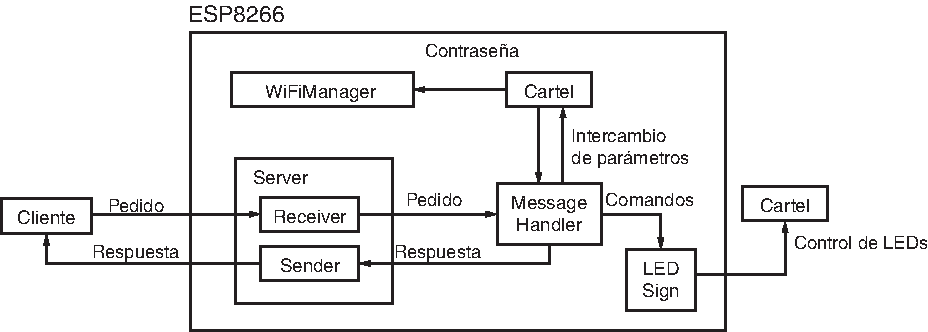
\includegraphics[width=1\linewidth]{imagenes/diagrama-bloque.pdf}
	\caption{Flujo de datos del lado del microcontrolador.}
	\label{fig:flujo_de_datos}
\end{figure}

A modo complementario se detalla un ejemplo relacionado a una secuencia de eventos que un cliente puede realizar.
En este caso, un usuario pide cambiar el texto que se muestra en la matriz. Este pedido es capturado por la clase Server quien le pasa la secuencia de bytes a MessageHandler.
Ésta interpreta la secuencia y obtiene el nuevo texto a representar. La información es enviada a LedSign quien desglosa el texto en letras y determina como deben encenderse las diferentes filas de la matriz de LEDs.
Por último, almacena el nuevo texto en la clase Settings para persistir la nueva información proporcionada.

A lo largo de la sección \ref{sec:sw-implementacion} se detalla cada clase mencionada, mostrando cuáles son sus interfaces de software y la forma en que se interconectan entre ellas.

\subsection{Aplicación de PC}

La aplicación de PC es la que utilizará el usuario para manejar el contenido (texto) del cartel y su configuración. La aplicación tendrá una interfaz gráfica de usuario para simplificar su uso.

\subsubsection{Requerimientos del software}\label{sec:sw-pc-req}
A continuación se enumera los requerimientos funcionales de este aplicativo:

\begin{itemize}
	\item Debe presentar al usuario un diálogo de login, para que él pueda ingresar la contraseña. Se puede ver en la figura \ref{fig:skgui-login} un bosquejo de este diálogo.
	\item Si la contraseña es incorrecta, se vuelve a mostrar el diálogo de login hasta que se ingrese la contraseña correcta o el usuario presione \enquote{Cancelar}.
	\item Debe permitir al usuario modificar el texto del cartel.
	\item Debe permitir al usuario modificar la configuración de red del cartel, es decir, los datos de la red Wi-Fi a la que se conecta al encenderse.
	\item Debe permitir al usuario modificar la contraseña de acceso al cartel.
	\item Mientras una comunicación con el cartel esté en curso, el usuario no debe poder realizar ninguna acción.
	\item Se debe poder ejecutar multiples instancias de la aplicación. Esto es útil para casos en que se quiera administrar mas de un cartel.
\end{itemize}

A continuación se listan los requerimientos no funcionales:
\begin{itemize}
	\item La aplicación deberá poder ejecutarse en Windows 7 o versiones posteriores.
	\item Al realizar operaciones de comunicación con el cartel, la aplicación no deberá dejar de responder a eventos de usuario.
	\item La aplicación deberá responder a acciones del usuario en un tiempo razonable, no más de un segundo (mostrar un cartel que indica operación en curso califica como responder).
\end{itemize}

\subsubsection{Interfaz de usuario}
Considerando los requisitos explícitados en la sección \ref{sec:sw-pc-req}, se armaron bosquejos de las distintas ventanas que conforman la interfaz de usuario del sistema.

\subsubsection{Ventana de login}
Esta ventana es la que aparece inmediatamente después de arrancar la ejecución del programa. Tiene un campo en que se ingresa el nombre de host del cartel (o directamente la IP) y un campo donde se ingresa la contraseña del cartel. Presionar \enquote{Conectar} debe iniciar la interacción de autenticación con el cartel y presionar \enquote{Cancelar} debe cerrar el programa. Se puede ver un bosquejo de esta ventana en la figura \ref{fig:skgui-login}.

\begin{figure}
	\centering
	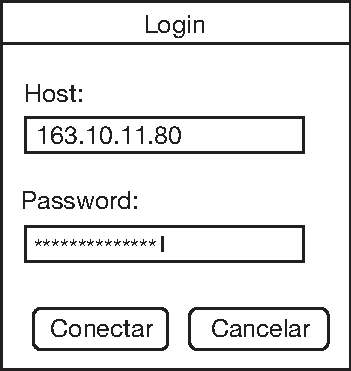
\includegraphics[scale=0.8]{imagenes/skgui-login.pdf}
	\caption{Bosquejo de la ventana de login.}
	\label{fig:skgui-login}
\end{figure}

\subsubsection{Ventana principal}

Esta ventana es con la cual usuario controla el cartel. Los elementos principales son:

\begin{itemize}
	\item Un campo de texto editable en el cual usuario ingrese el texto a mostrar.
	\item Un casilla de verificación que habilite o deshabilite el parpadeo.
	\item Un campo numérico editable para establecer la frecuencia de parpadeo. Este campo solo debe estar activo si estuviera tildada su casilla de verificación correspondiente.
	\item Un casilla de verificación que habilite o deshabilite el deslizamiento.
	\item Un campo numérico editable para establecer la velocidad de deslizamiento. Este campo solo debe estar activo si estuviera tildada su casilla de verificación correspondiente.
	\item Un botón \enquote{Aplicar} que inicia la comunicación con el cartel, con el objeto de actualizar el texto del cartel con el texto que ingresó el usuario en el campo, junto a los parámetros de animación (parpadeo y deslizamiento).
	\item Un botón \enquote{Restaurar} que inicia comunicación con el cartel con el objeto de traer los datos (texto y configuración) del cartel a la aplicación de PC, descartando todo cambio que el usuario haya hecho pero no aplicado.
\end{itemize}

Todos estos elementos se pueden ver en el bosquejo que muestra la figura \ref{fig:skgui-principal}.

\begin{figure}
	\centering
	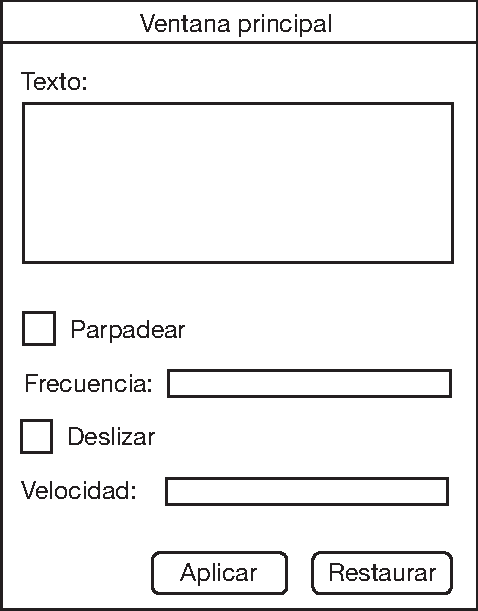
\includegraphics[scale=0.8]{imagenes/skgui-principal.pdf}
	\caption{Bosquejo de la ventana principal.}
	\label{fig:skgui-principal}
\end{figure}

\subsubsection{Ventana de configuración}
La ventana de configuración es la que utilizará el usuario para cambiar los parámetros de la red WiFi a la cual se deberá conectar el cartel la próxima vez que arranque o se reinicie. En ella se tiene un campo para ingresar el nombre de la red (SSID), un campo para ingresar la contraseña de la red, un botón \enquote{Modificar} y un botón \enquote{Cancelar}.

El botón \enquote{Modificar} debe cerrar la ventana e iniciar la interacción con el cartel para actualizar la configuración, mientras que el botón \enquote{Cancelar} debe volver a la ventana principal sin realizar ningún cambio y descartar los datos ingresados.

Esta ventana será alcanzable desde un menú ubicado en la ventana principal.

Todos estos elementos se pueden ver en el bosquejo que muestra la figura \ref{fig:skgui-conf}.

\begin{figure}
	\centering
	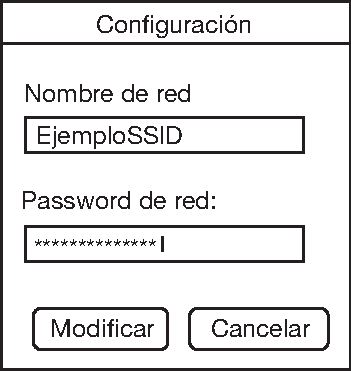
\includegraphics[scale=0.8]{imagenes/skgui-conf.pdf}
	\caption{Bosquejo de la ventana de configuración de red WiFi.}
	\label{fig:skgui-conf}
\end{figure}

\subsubsection{Ventana de cambio de contraseña}
Esta ventana es en la cual el usuario ingresa la contraseña nueva para que el cartel tome como correcta a partir de esta operación.

Es importante notar que esta operación no se puede realizar si el usuario ni hubiese ingresado anteriormente la contraseña correcta. De hecho, el usuario no puede realizar ni esta ni ninguna otra operación, quedando estancado en la ventana de login, como se especificó en los requerimientos funcionales.

Esta ventana será alcanzable desde un menú ubicado en la ventana principal.

Se puede ver un bosquejo de la ventana de cambio de contraseña en la figura \ref{fig:skgui-passwd}

\begin{figure} [h!]
	\centering
	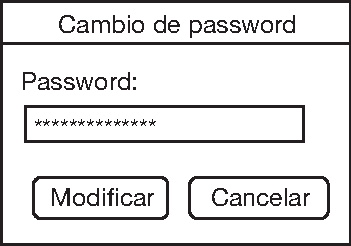
\includegraphics[scale=0.8]{imagenes/skgui-passwd.pdf}
	\caption{Bosquejo de la ventana de cambio de contraseña.}
	\label{fig:skgui-passwd}
\end{figure}

\subsubsection{Arquitectura del software}
Al tratarse de una aplicación con interfaz gráfica de usuario, resulta útil tomar un paradigma de programación basada en eventos. Esto combina bien con la programación orientada a objetos. Un patrón de arquitectura de software muy conocido es el patrón Model-View-Controller (MVC).

El patrón MVC \cite{MVC} tiene como objetivo principal el de desacoplar el manejo de datos de la interfaz de usuario, de manera que se logre mejor eficiencia en el resuso del código y el desarrollo en simultáneo entre mas de una persona. Es un patrón que expresa el núcleo de la arquitectura, dejando abierta la posibilidad de cambio y adaptación del patrón a cada problema particular. Es muy utilizado en aplicaciones con interfaz gráfica de usuario.

\begin{figure} [h!]
	\centering
	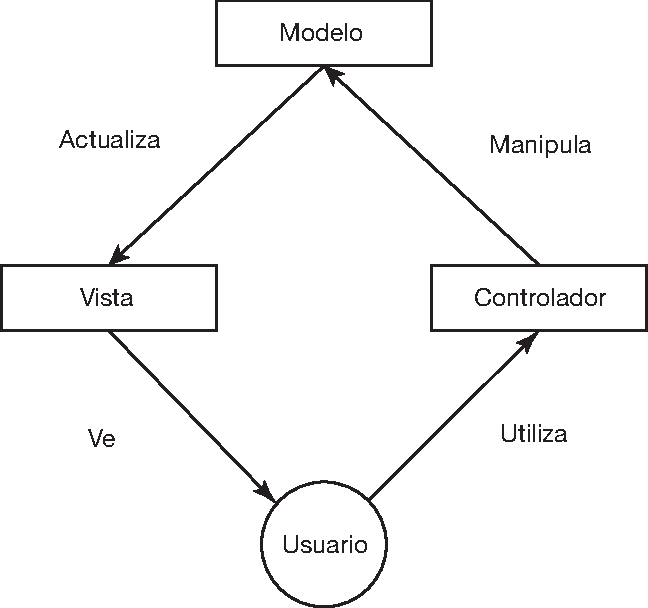
\includegraphics[scale=0.8]{imagenes/mvc.pdf}
	\caption{Arquitectura de software Model-View-Controller.}
	\label{fig:mvc}
\end{figure}

En el patrón MVC, se separan los objetos de forma que caigan en una de tres categorías:
\begin{description}
	\item[Modelo: ] Encapsula los datos. En este caso, esos datos pueden ser el texto del cartel junto a sus parámetros de animación, o la configuración de red del cartel. De haber modificaciones, actualiza la vista para reflejar estos cambios.
	\item[Vista: ] Representa a la interfaz gráfica que el usuario ve.
	\item[Controlador: ] Hace de mediador entre el modelo y la vista. Toma los eventos de interfaz de usuario y actúa sobre ellos, manipulando el modelo si fuera necesario.
\end{description}

Se puede ver en la figura \ref{fig:mvc} un gráfico resumiendo el rol del Modelo, Vista y Controlador.


\FloatBarrier
\subsection{Protocolo de comunicación de red} \label{sec:protocolo}

\subsubsection{Codificación}

Cada mensaje del protocolo es un paquete de tamaño fijo de tamaño igual a 256 bytes.
Dentro de esa longitud está incluido el header.
Todos los valores numéricos se transmiten con orden de bytes Big-Endian.
Cada mensaje respeta un formato base común. Se puede ver este formato en la figura \ref{fig:paquete-base}.


\begin{figure}[!ht]
	\centering
	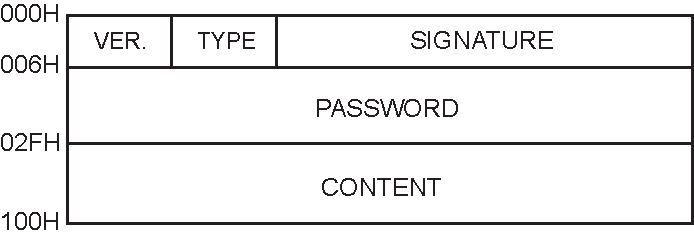
\includegraphics[width=0.6\linewidth]{imagenes/protocolo/paquete-base.pdf}
	\caption{Esquema general entre todos los componentes del sistema.}
	\label{fig:paquete-base}
\end{figure}

\begin{itemize}
	\item version: es un número de 8 bits que identifica la versión del protocolo, por si se hicieran cambios y se quiera mantener retrocompatibilidad.
	\item type: es un enumerativo que codifica el tipo de mensaje. Más adelante se detalla los diferentes tipos posibles.
	\item signature: es una palabra de 4 caracteres que siempre tiene que ser ANRS.
	\item password: es la contraseña del sistema. Debe incluirse en cada paquete que se envía hacia el microcontrolador. Los paquetes que envía éste como respuesta dejan dicho campo vacío.
	\item content: es una estructura cuya interpretación depende de type y se define más adelante.
\end{itemize}



\subsubsection{Interacción}

El primer paso para comenzar una interacción debe hacerla el cliente, iniciando una conexión TLS con el servidor.
A continuación, el usuario envía un mensaje denominado request y que puede tomar alguno de los siguiente valores en su campo type.

\begin{itemize}
	\item SetPassword: establece una nueva contraseña del sistema.
	\item GetText: pide, al servidor, el contenido del cartel, su velocidad de parpadeo y desplazamiento.
	\item SetText: establece el nuevo contenido del cartel, su velocidad de parpadeo y desplazamiento.
	\item GetWiFiConfig: pide, al servidor, la configuración WiFi relacionada a la red a la que actualmente se encuentra conectado el microcontrolador.
	\item SetWiFiConfig: establece la nueva configuración WiFi respecto de la nueva red a la que el microcontrolador debe conectarse la próxima vez que se inicie el sistema.
\end{itemize}

Así mismo, el cliente, debe especificar la versión de protocolo que utiliza, la firma y la contraseña del sistema.
Por su parte, el servidor, recibe el paquete, analiza todos los campos del header y emite una respuesta hacia el cliente de acuerdo al pedido realizado por éste.
El campo type de la respuesta puede obtener los siguientes valores.

\begin{itemize}
	\item GetTextResponse: envía hacia el usuario la información del contenido y los parámetros de configuración del cartel.
	\item GetWiFiConfigResponse: envía hacia el usuario la información respecto de la red WiFi a la que actualmente se encuentra conectado el servidor.
	\item GenericResponse: es un tipo de paquete que se envía de vuelta, cuando alguno de los datos proporcionados por el cliente no son válido.
\end{itemize}

Respecto de este último tipo de mensajes, los códigos de respuesta posibles son los que se listan a continuación.

\begin{itemize}
	\item OK: se envía ante un pedido de cambio de algún parámetro enunciado previamente, cuando la operación fue realizada satisfactoriamente.
	\item MalformedPacket: se envía cuando el paquete recibido de parte del cliente contiene una firma o un tipo inválido.
	\item BadPassword: se envía cuando la contraseña proporcionada por parte del cliente es incorrecta.
	\item BadProtocolVersion: se envía cuando el protocolo del programa es superior al que soporta el servidor.
	\item BadIP: se envía cuando la nueva ip proporcionada es incorrecta.
	\item BadSubnetMask: se envía cuando la nueva máscara de red proporcionada es incorrecta.
\end{itemize}

Luego de obtener la respuesta, el cliente debe cerrar la conexión inmediatamente.
De esta forma se completa una interacción entre el usuario y servidor.
En caso de que la conexión no fuera cerrada por el usuario, el servidor pasado un cierto tiempo la finaliza.
A lo largo de esta sección se detallan las distintas estructuras del campo content, de forma de mostrar a qué corresponde cada campo.



\subsubsection{SetPassword}

El paquete de este tipo permite cambiar la contraseña del sistema.
En content se encuentra la nueva contraseña, tiene un máximo de 40 caracteres sin incluir al caracter nulo.
La respuesta que se recibe es del tipo GenericResponse.



\subsubsection{GetText}

El paquete de este tipo permite obtener el contenido actual del cartel, así como también sus configuraciones relacionadas a la velocidad de parpadeo y desplazamiento del mensaje.
El campo content queda vacío puesto que su contenido no es utilizado para procesar la petición.

Se espera una respuesta del servidor del tipo GetTextResponse donde el contenido posee toda la información previamente mencionada.



\subsubsection{SetText}

El paquete de este tipo permite establecer un nuevo mensaje a representar en el cartel, así como también sus parámetros de configuración.
El campo content debe respetar la estructura que se observa en la figura \ref{fig:paquete-anim}


\begin{figure}[!ht]
	\centering
	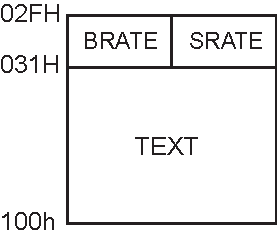
\includegraphics[width=0.3\linewidth]{imagenes/protocolo/paquete-anim.pdf}
	\caption{Esquema general entre todos los componentes del sistema.}
	\label{fig:paquete-anim}
\end{figure}

BRATE y SRATE son la frecuencia de parpadeo en Hz y la velocidad de deslizamiento en píxeles por segundo.
Se asume que si BRATE es cero, no se debe parpadear el contenido.
De la misma forma, si SRATE es cero, no se debe deslizar el contenido.
El tipo de dato ufp844 es un número en punto fijo sin signo con 4 bits de parte entera y 4 bits de parte fraccionaria.
El tipo de dato sfp844 es lo mismo que ufp844 pero en complemento a dos.
Por último, en content se encuentra el campo text asociado al mensaje a mostrar en el cartel.
El mismo debe tener un terminador nulo para indicar el fin del contenido.
La respuesta que se recibe es del tipo GenericResponse.



\subsubsection{GetWiFiConfig}

El paquete de este tipo permite obtener el SSID, contraseña WiFi, ip y máscara de subred respecto de la red a la que actualmente se encuentra cnectado el servidor.
El campo content queda vacío puesto que su contenido no es utilizado para procesar la petición.

Se espera una respuesta del servidor del tipo GetWiFiConfigResponse donde el contenido posee toda la información previamente mencionada.



\subsubsection{SetWiFiConfig}

El paquete de este tipo permite establecer un nuevo SSID, contraseña WiFi, ip y máscara subred respeco de la red que se conectará la próxima vez que se incie el sistema.
El campo content debe respetar la estructura que se observa en la figura \ref{fig:paquete-wifi}


\begin{figure}[!ht]
	\centering
	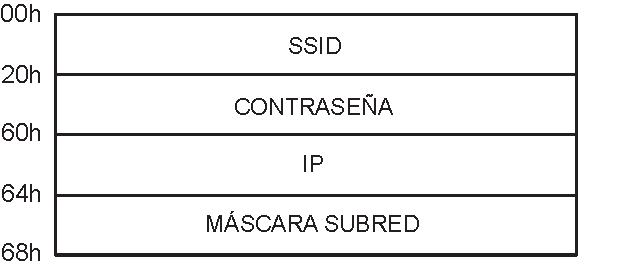
\includegraphics[width=0.5\linewidth]{imagenes/protocolo/paquete-wifi.pdf}
	\caption{Esquema general entre todos los componentes del sistema.}
	\label{fig:paquete-wifi}
\end{figure}

La respuesta que se recibe es del tipo GenericResponse.


\subsubsection{Strings}

Los strings tienen un límite de longitud dado por el lugar remanente en el mensaje y están codificados según el estándar ISO/IEC 8859-1:1998.
El último byte del contenido, es necesario colocar un caracter nulo de modo que indique el final de la cadena de texto.


\subsubsection{Sobre Transport Security Layer}\label{sec:tls}
En este apartado se discutirá brevemente sobre el protocolo de red TLS, que es utilizado en este proyecto para lograr una conexión cifrada y autenticada. Esta sección tiene como objetivo explicar al lector la necesidad y la importancia de la generación de certificados TLS, proceso que se realiza en la guía de puesta en marcha.

El protocolo TLS está diseñado para permitir a aplicaciones con arquitectura de cliente-servidor comunicarse de manera que se evita las escuchas por terceros, alteración o falsificación de datos\cite{TLS}. Esto resulta crítico para este proyecto ya que el usuario de cartel debe ingresar una contraseña de forma remota; si la conexión no fuera resistente a escuchas, entonces un atacante podría capturar la contraseña sin conocimiento del usuario legítimo y conseguir acceso al cartel.

Los objetivos del protocolo TLS son los siguientes:
\begin{description}
	\item [Seguridad criptográfica:] TLS se utiliza para establecer una conexión segura entre dos partes.
	\item [Interoperabilidad:] Dos o más programadores independientes deberían poder desarrollar aplicaciones utilizando TLS que puedan intercambiar parámetros criptográficos sin tener conocimiento del código de la otra aplicación.
	\item [Extensibilidad:] TLS busca proveer un marco al cual se le pueden incorporar nuevos algoritmos de cifrado. Esto tiene como resultado el hecho de que al agregar un nuevo algoritmo no es necesario crear un nuevo protocolo y, por lo tanto, una nueva implementación.
	\item [Eficiencia relativa:] Las operaciones criptográficas tienden a ser intensivas en cómputo, especialmente las operaciones que trabajan sobre las claves públicas. Para esto el protocolo TLS especifica un mecanismo de cacheo de sesiones para reducir el número de conexiones que se debe establecer desde cero. Por otro lado, se tomaron medidas para reducir el uso de ancho de banda en la red.
\end{description}

\subsection{Criptografía asimétrica}
La criptografía asimétrica o criptografía de clave pública es cualquier sistema criptográfico que utiliza pares de claves: claves públicas que se distribuyen ampliamente y claves privadas que son conocidas únicamente por su dueño. 

Esto logra la autenticación, es decir, que la clave pública verifique que el dato haya sido cifrado utilizando la clave privada. Haciendo esto también se obtiene el cifrado del mensaje, que implica que sólo la clave privada es capaz de decifrar el dato cifrado con la clave pública \cite{crypto}.

En este sistema criptográfico, cualquiera puede cifrar un dato arbitrario (texto plano a partir de ahora)\footnote{Se utiliza en este texto el término texto plano para cualquier dato, no necesariamente debe ser texto bajo alguna codificación como ASCII, UTF-8, etc.} con la clave pública (ya que esta disponible a cualquiera) y ese dato cifrado (texto cifrado a partir de ahora) sólo se puede obtener utilizando la clave privada para decifrarlo.

En general, los algoritmos de cifrado utilizados en sistemas de clave asimétrica son computacionalmente intensos, por lo cual TLS los utiliza únicamente para el establecimiento seguro de una clave en común a las partes. Esta clave común luego se utiliza para cifrar el resto de los datos que circulan por la conexión utilizando cifrado simétrico (un mensaje se cifra con una clave y se decifra con la misma), que es menos computacionalmente intenso.

El proceso que establece la clave en común se denomina \emph{handshake}. Este procedimiento se realiza al comienzo de una conexión TLS.

En el contexto del sistema de este proyecto, el cartel es el servidor y es quien debe tener la clave pública y la clave privada mientras que el cliente no necesita tener un elemento del sistema criptográfico.

Sin embargo, esta situación tal como está planteada no resuelve el problema de la identificación del cartel, es decir, el cliente puede conectarse al cartel con la idea de que se trata del cartel al que se quiere conectar, y el cartel puede ser en realidad un atacante haciéndose pasar por el cartel, con la intención de capturar la contraseña. Este problema se resuelve simplemente incrustando a priori a la aplicación de PC la clave pública del cartel legítimo. De esta forma, el cliente (la aplicación de PC) aborta el \emph{handshake} si las firmas públicas no coinciden. El atacante posiblemente tenga en su poder la clave pública del cartel legítimo pero no su clave privada correspondiente, sin la cual no se puede realizar el \emph{handshake}, porque en algún punto del transcurso de éste, el cliente cifrará un mensaje con la clave pública y el atacante no tendrá la clave privada para decifrarlo.